%\documentclass{beamer}
\documentclass[xcolor=table]{beamer}
%%%%%%%%%%%%%%%%%%%%%%%%%%%%%%%%%%%%%%%%%%%%%%%%%%%%%%%%%%%%%%%%%%%%%%%%%%%%%%%%%%%%%%%%%%%%%%%%%%%%%%%%%%%%%%%%%%%%%
% Cada tema possui uma estrutura de apresentação e formatação de cores e 
% fontes específica, assim podemos escolher aquele que seja mais adequado à nossa apresentação:

% Antibes, Bergen, Berkeley, Berlin, Boadilla, Copenhagen, Darmstadt, Dresden, Frankfurt,
% Goettingen, Hannover, Ilmenau, Juanlespins, Madrid, Malmoe, Montpellier, Paloalto, Pittsburgh, Rochester e Singapore

%%%%%%%%%%%%%%%%%%%%%%%%%%%%%%%%%%%%%%%%%%%%%%%%%%%%%%%%%%%%%%%%%%%%%%%%%%%%%%%%%%%%%%%%%%%%%%%%%%%%%%%%%%%%%%%%%%%%%%
%\usetheme{Boadilla} 
%%%%%%%%%%%%%%%%%%%%%%%%%%%%%%%%%%%%%%%%%%%%%%%%%%%%%%%%%%%%%%%%%%%%%%%%%%%%%%%%%%%%%%%%%%%%%%%%%%%%%%%%%%%%%%%%%%%%%%
% Modelos de Slides:
% AnnArbor, 

% Tipos de Cores:
% default, albatross, beaver, beetlebeetle, crane, dolphin, dove, fly, lily, orchid, rose, seagull, seahorse, whale, wolverine.
%%%%%%%%%%%%%%%%%%%%%%%%%%%%%%%%%%%%%%%%%%%%%%%%%%%%%%%%%%%%%%%%%%%%%%%%%%%%%%%%%%%%%%%%%%%%%%%%%%%%%%%%%%%%%%%%%%%%%%
% Tema, cor e fonte modo matematico
\usetheme{Madrid}  % modelo de slides...
\usecolortheme{whale}   % tipo de cores..
\usefonttheme[onlymath]{serif}   % Veja mais temas e cores em http://www.hartwork.org/beamer-theme-matrix/

\usefonttheme[onlylarge]{structurebold}
\setbeamerfont*{frametitle}{size=\normalsize,series=\bfseries} 
\setbeamertemplate{navigation symbols}{}  % Retira os simbolos.
%%%%%%%%%%%%%%%%%%%%%%%%%%%%%%%%%%%%%%%%%%%%%%%%%%%%%%%%%%%%%%%%%%%%%%%%%%%%%%%%%%%%%%%%%%%%%%%%%%%%%%%%%%%%%%%%%%%%%%
\newtheorem{teo}{Teorema}[section]

%%%%%%%%%%%%%%%%%%%%%%%%%%%%%%%%%%%%%%%%%%%%%%%%%%%%%%%%%%%%%%%%%%%%%%%%%%%%%%%%%%%%%%%%%%%%%%%%%%%%%%%%%%%%%%%%%%%%%%%%%%%%%%%%5
% Pacotes padrão:
\usepackage[brazil]{babel}  
\usepackage[utf8]{inputenc}
\usepackage{default}
\usepackage{times}
\usepackage[T1]{fontenc}
\usepackage{ae}                                        
\usepackage{microtype}                                 
\usepackage{amsfonts}
\usepackage{float}
\usepackage{amsmath,amssymb}                         
\usepackage{xcolor}                                  
\usepackage{color,colortbl,multirow}                 
\usepackage{multicol}                                
\usepackage{enumerate,hyperref}
\usepackage{palatino}	
\usepackage{keyval}
\usepackage{subcaption}
\usepackage{xfrac}  
\usepackage{pdfpages}
%\usepackage[pdftex,plainpages=false,pdfpagelabels,pagebackref,colorlinks=true,citecolor=green,linkcolor=black,urlcolor=black,filecolor=black,bookmarksopen=true]{hyperref}


\usepackage{animate}
\usepackage{multimedia}

%%%%%%%%%%%%%%%%%%%%%%%%%%%%%%%%%%%%%%%%%%%%%%%%%%%%%%%%%%%%%%%%%%%%%%%%%%%%%%%%%%%%%%%%%%%%%%%%%%%%%
% Setup TikZ
\usepackage{tikz}                                     
\usetikzlibrary{arrows}
\tikzstyle{block}=[draw opacity=0.7,line width=1.4cm]

\newcommand{\nvec}{\mathbf{n}}
\newcommand{\xvec}{\mathbf{x}}
\newcommand{\evec}{\mathbf{e}}
\newcommand{\vvec}{\mathbf{v}}
\newcommand{\mvec}{\mathbf{m}}
\newcommand{\uvec}{\mathbf{u}}
\newcommand{\fvec}{\mathbf{f}}
\newcommand{\zvec}{\mathbf{0}}
\newcommand{\Psivec}{\mathbf{ \Psi}}
\newcommand{\xivec}{\boldmath \xi}

%%%%%%%%%%%%%%%%%%%%%%%%%%%%%%%%%%%%%%%%%%%%%%%%%%%%%%%%%%%%%%%%%%%%%%%%%%%%%%%%%%%%%%%%%%%%%%%%%%%%%
% Logo tipo:
% O comando pgfdeclareimage associa um arquivo de imagem com um identificador (neste caso, logo). % Formatos válidos de imagem são JPG, PNG e PDF.
%\pgfdeclareimage[width=0.8cm,height=1.2cm]{logo}{ufpa} 
%\logo{\pgfuseimage{logo}}

% Titulo, autor, instituição:
\title[]{}
\author[]{}
%\institute{UFPA}
\date{17/03/2021}

%logo in the first page only:
%   \logo{\includegraphics[width=2.5cm]{cnpq.png}\hspace*{5cm}}   
%%%%%%%%%%%%%%%%%%%%%%%%%%%%%%%%%%%%%%%%%%%%%%%%%%%%%%%%%%%%%%%%%%%%%%%%%%%%%%%%%%%%%%%%%%%%%%%%%%%%%%%%%%
% Tela cheia
\hypersetup{pdfpagemode=FullScreen}

%%%%%%%%%%%%%%%%%%%%%%%%%%%%%%%%%%%%%%%%%%%%%%%%%%%%%%%%%%%%%%%%%%%%%%%%%%%%%%%%%%%%%%%%%%%%%%%%%%%%%%%%%%%
%%%%%%%%%%%%%%%%%%%%%%%%%%%%%%%%%%%%%%%%%%%%%%%%%%%%%%%%%%%%%%%%%%%%%%%%%%%%%%%%%%%%%%%%%%%%%%%%%%%%%%
%It's also possible to put the table of contents at the beginning of each section and highlight the title of the current section.
%\AtBeginSection[]
%{
%\begin{frame}
%\frametitle{Sum\'ario}
%\tableofcontents[currentsection]
%\end{frame}
%}
%%%%%%%%%%%%%%%%%%%%%%%%%%%%%%%%%%%%%%%%%%%%%%%%%%%%%%%%%%%%%%%%%%%%%%%%%%%%%%%%%%%%%%%%%%%%%%%%%%%%%
\begin{document}
%\justifying % Paragrafo justificado
\begin{frame}
%  \cape
  \titlepage
\end{frame}

%\begin{frame}\frametitle{Sum\'ario}
%  \tableofcontents
%\end{frame}

%\begin{frame}
%\frametitle{Sum\'ario}
%\tableofcontents[currentsection]
%\end{frame}

%\section{Introdu\c{c}\~ao} %%%%%%%%%%%%%%%%%%%%%%%%%%%%%%%%%%%%%%%%%%%%%%%%%%%%%%%%%%%%%%%%%%%%%%%%%%%%%%%%%%%%%%%%%%%%%%%%%%%%%%%%%%%%                                 

%%%%%%%%%%%%%%%%%%%%%%%%%%%%%%%%%%%%%%%%%%%%%%%%%%%%%%%%%%%%%%%%%%%%%%%%%%%%%%%%%%%%%%%%%%%%%%%%%%%%%%%%%%%%%%%%%%%%%%%%%%%%%%%%%%%%%%%%%%%%%%%%%
%%%%%%%%%%%%%%%%%%%%%%%%%%%%%%%%%%%%%%%%%%%%%%%%%%%%%%%%%%%%%%%%%%%%%%%%%%%%%%%%%%%%%%%%%%%%%%%%%%%%%%%%%%%%%%%%%%%%%%%%%%%%%%%%%%%%%%%%%%%%%%%%55


\begin{frame}
\frametitle{\textbf{Solu\c{c}\~ao para a fun\c{c}\~ao de Green em um meio homog\^eneo, isotr\'opico e ilimitado}}
    
\begin{flushleft}
Encontrar a solu\c{c}\~ao da equa\c{c}\~ao da onda da elastodin\^amica, 
\end{flushleft}
\begin{eqnarray}
  \label{ten1}
      \partial_{tt}\uvec(\xvec,t) &=& \left(\lambda + \mu\right) \nabla \left(\nabla \cdot \uvec \right) - \mu\nabla \times \left(\nabla \cdot \uvec \right)  + \fvec(\xvec,t)\, 
\end{eqnarray}
\begin{flushleft}
para uma distribui\c{c}\~ao de fontes com depend\^encia temporal
\end{flushleft}
\begin{equation}
  \label{ten1}
      \fvec(\xvec,t) = X_{0}(t)\delta(\xvec)\evec_1\, .
\end{equation}
\begin{flushleft}
\textcolor{red}{Passo 1}:\hspace{0.025cm} escrever a for\c{c}a de corpo em potenciais de Hemholtz,\\
$\Phi(\xvec,t)$ potencial de fonte escalar e \\
$\Psi(\xvec,t)$ potencial de fonte vetorial.\\
\end{flushleft}
\begin{equation}
  \label{ten1}
      \fvec(\xvec,t) = X_{0}(t)\delta(\xvec)\evec_1 = \nabla \Phi + \nabla \times \Psi \quad\quad \mbox{e} \quad\quad    \nabla \cdot \Psi(\xvec,t) = 0 \, .
\end{equation}

\end{frame}%%%%%%%%%%%%%%%%%%%%%%%%%%%%%%%%%%%%%%%%555



\begin{frame}
\frametitle{\textbf{Solu\c{c}\~ao para a fun\c{c}\~ao de Green em um meio homog\^eneo, isotr\'opico e ilimitado}}

\begin{flushleft}
Recorremos a solu\c{c}\~ao da equa\c{c}\~ao de Poisson para $\fvec(\xvec,t)$,
\end{flushleft}   
\begin{equation*}
  \label{ten1}
      \fvec(\xvec,t) = X_{0}(t)\delta(\xvec)\evec_1 = \nabla \Phi + \nabla \times \Psi \quad\quad \mbox{e} \quad\quad    \nabla \cdot \Psi(\xvec,t) = 0 \, .
\end{equation*}
\begin{flushleft}
Um termo de fonte
\end{flushleft}
\begin{equation*}     
 \mathbf{Z(\xvec,t)} = \nabla X(\xvec,t) + \nabla \times \mathbf{Y}(\xvec,t) \qquad \mbox{e} \qquad
 \nabla \cdot \mathbf{Y} = 0
\end{equation*}
\begin{flushleft}
A solu\c{c}\~ao da equa\c{c}\~ao de Poisson,
\end{flushleft}       
\begin{align*}     
 \nabla^2 \mathbf{W}(\xvec,t) =&  \mathbf{Z}(\xvec,t)\, 
\end{align*}  
\begin{flushleft}  
\'e dada por
\end{flushleft}
\begin{eqnarray}
  \label{ten1}
     \mathbf{W}(\xvec,t) &=& - \frac{1}{4\pi} \int_{V} \frac{\mathbf{Z}(\xvec,t)}{\left| \xvec - \xivec \right|} dV(\xivec)\, .
 \end{eqnarray}
\begin{flushleft}
Com os potenciais de Hemholtz $X(\xvec,t)$ e $\mathbf{Y}(\xvec,t)$:
\end{flushleft}
\begin{equation*}          
    X(\xvec,t) = \nabla \cdot \mathbf{W}(\xvec,t) \qquad \mbox{e } \qquad
   \mathbf{Y}(\xvec,t) =- \nabla \times \mathbf{W}(\xvec,t)\, .
\end{equation*}         
 
\end{frame}%%%%%%%%%%%%%%%%%%%%%%%%%%%%%%%%%%%%%%%%555


\begin{frame}
\frametitle{\textbf{Solu\c{c}\~ao para a fun\c{c}\~ao de Green em um meio homog\^eneo, isotr\'opico e ilimitado}}

\begin{flushleft}
Substituindo $\mathbf{Z}$ por $X_{0}(t)\delta(\xvec)\evec_1$ a solu\c{c}\~ao da equa\c{c}\~ao de Poisson 
para esse termo de fonte \'e obtida por compara\c{c}\~ao:
\end{flushleft}
\begin{eqnarray}
  \label{ten1}
     \mathbf{W} &=& - \frac{X_{0}(t)}{4\pi} \int_{V} \frac{\delta(\xivec) (1,0,0)}{\left| \xvec - \xivec \right|} dV =  - \frac{X_{0}(t)}{4\pi\left| \xvec \right|}{×} \evec_1\,  .
 \end{eqnarray}
\begin{flushleft}
Determinamos os potenciais de Hemholtz que comp\~oe a fonte $\fvec(\xvec,t)$,    
 \end{flushleft}
\begin{eqnarray}
  \label{ten1}
      \Phi(\xvec,t) &=& \nabla \cdot \mathbf{W} = \frac{\partial }{\partial x_1} \left( -\frac{X_{0}(t)}{4\pi\left| \xvec \right|} \right) = - \frac{X_{0}(t)}{4\pi} \frac{\partial }{\partial x_1} \frac{1}{\left| \xvec \right|} \, \\ 
      \Psi(\xvec,t) &=& - \nabla \times \mathbf{W} =  \frac{X_{0}(t)}{4\pi}\left(0, \frac{\partial }{\partial x_3}  \frac{1}{\left| \xvec \right|},-\frac{\partial }{\partial x_2} \frac{1}{\left| \xvec \right|}  \right)\, .
\end{eqnarray}
    
\end{frame}%%%%%%%%%%%%%%%%%%%%%%%%%%%%%%%%%%%%%%%%55




\begin{frame}
\frametitle{\textbf{Solu\c{c}\~ao para a fun\c{c}\~ao de Green em um meio homog\^eneo, isotr\'opico e ilimitado}}

\begin{flushleft}
 \textcolor{red}{Passo 2}:\hspace{0.025cm} encontrar os potenciais de deslocamento de onda de Lam\'e $\phi(\xvec,t)$ e $\psi(\xvec,t)$ \'e resolver equa\c{c}\~oes do tipo:\\ 
\end{flushleft}
\begin{itemize}
  \item para a equa\c{c}\~ao do potencial escalar de onda P: 
 \end{itemize} 
\begin{eqnarray}
  \label{ten1}  
       \frac{\partial^2 \phi(\xvec,t)}{\partial t^2} &=& \alpha \nabla^2 \phi(\xvec,t) + \frac{\Phi(\xvec,t)}{\rho} \, .
 \end{eqnarray}
 
\begin{flushleft}
Tento solu\c{c}\~ao geral para uma distribui\c{c}\~ao de fonte volum\'etrica dependente do tempo,
\end{flushleft}
\begin{eqnarray}
 \Phi(\xvec,t) &=&  \int_{-\infty}^{+\infty}\, d\tau \int_{V} \Phi(\xivec,\tau)\delta(\xvec -\xivec)\delta(t -\tau) dV(\xivec)\, ,
\end{eqnarray}
\begin{flushleft}
da forma
\end{flushleft}
\begin{eqnarray}
 \phi(\xvec,t) &=& \frac{1}{4\pi\alpha^{2} \rho} \int_{V} \frac{ \Phi \left( \xivec,t - \frac{\left|\xvec - \xivec \right|}{\alpha}  \right) }{\left|\xvec - \xivec \right|} dV(\xivec)\, .
\end{eqnarray} 
 
\end{frame}%%%%%%%%%%%%%%%%%%%%%%%%%%%%%%%%%%%%%%%%555



\begin{frame}
\frametitle{\textbf{Solu\c{c}\~ao para a fun\c{c}\~ao de Green em um meio homog\^eneo, isotr\'opico e ilimitado}}

\begin{flushleft}
O deslocamento de potencial de onda P, $\phi(\xvec,t)$, para o potencial de fonte escalar 
\end{flushleft}
\begin{eqnarray}
  \label{ten1}
      \Phi(\xvec,t) &=& - \frac{X_{0}(t)}{4\pi} \frac{\partial }{\partial x_1} \frac{1}{\left| \xvec \right|} \, 
\end{eqnarray}

\begin{flushleft} 
\'e encontrado substituindo-o na equa\c{c}\~ao de potencial escalar de onda P,
\end{flushleft}
\begin{eqnarray}
  \label{ten1}
       \frac{\partial^2 \phi(\xvec,t)}{\partial t^2} &=& \alpha \nabla^2 \phi(\xvec,t) - \frac{1}{\rho}\frac{X_{0}(t)}{4\pi} \frac{\partial }{\partial x_1} \frac{1}{\left| \xvec \right|} \,       
\end{eqnarray}
\begin{flushleft}
a solu\c{c}\~ao $\phi(\xvec,t)$ segue
\end{flushleft}
\begin{eqnarray}
  \label{ten1}
       \phi(\xvec,t) &=& - \frac{1}{(4\pi\alpha)^{2} \rho} \int_{V} \frac{ X_{0} \left( \xivec,t - \frac{\left|\xvec - \xivec \right|}{\alpha}  \right) }{\left|\xvec - \xivec \right|} \frac{\partial }{\partial \xi_1} \frac{1}{\left| \xivec \right|} dV(\xivec)\,       
\end{eqnarray}


\end{frame}%%%%%%%%%%%%%%%%%%%%%%%%%%%%%%%%%%%%%%%%555




\begin{frame}
\frametitle{\textbf{Solu\c{c}\~ao para a fun\c{c}\~ao de Green em um meio homog\^eneo, isotr\'opico e ilimitado}}
\begin{flushleft}
 \textcolor{red}{Passo 2}:\hspace{0.025cm} encontrar os potenciais de deslocamento de onda de Lam\'e $\phi(\xvec,t)$ e $\psi(\xvec,t)$ \'e resolver equa\c{c}\~oes do tipo:\\ 
\end{flushleft}
\begin{itemize}
  \item para a equa\c{c}\~ao do potencial vetorial de onda S: 
 \end{itemize} 
\begin{eqnarray}
  \label{ten1}
       \frac{\partial^2 \psi(\xvec,t)}{\partial t^2} &=& \beta \nabla^2 \phi(\xvec,t) + \frac{\Psi(\xvec,t)}{\rho} \,        
 \end{eqnarray}
\begin{flushleft}
Resolver a equa\c{c}\~ao para o potencial de fonte vetrorial $\Psi(\xvec,t)$,
\end{flushleft}
\begin{eqnarray}
  \label{ten1}
       \frac{\partial^2 \psi(\xvec,t)}{\partial t^2} &=& \beta \nabla^2 \psi(\xvec,t) + \frac{1}{\rho}\frac{X_{0}(t)}{4\pi}\left(0, \frac{\partial }{\partial x_3}  \frac{1}{\left| \xvec \right|},-\frac{\partial }{\partial x_2} \frac{1}{\left| \xvec \right|}  \right) \, 
\end{eqnarray}
\begin{flushleft}
de forma an\'aloga a solu\c{c}\~ao $\psi(\xvec,t)$ \'e
\end{flushleft}
\begin{eqnarray}
  \label{ten1}
\psi(\xvec,t) &=& \frac{1}{(4\pi\beta)^{2} \rho} \int_{V} \frac{ X_{0} \left( \xivec,t - \frac{\left|\xvec - \xivec \right|}{\beta}  \right) }{\left|\xvec - \xivec \right|}  \left(0, \frac{\partial }{\partial \xi_3} \frac{1}{\left| \xivec \right|}, \frac{\partial }{\partial \xi_2} \frac{1}{\left| \xivec \right|} \right) dV(\xivec) \, \nonumber \\
\end{eqnarray}
       
\end{frame}%%%%%%%%%%%%%%%%%%%%%%%%%%%%%%%%%%%%%%%%555




\begin{frame}
\frametitle{\textbf{Solu\c{c}\~ao para a fun\c{c}\~ao de Green em um meio homog\^eneo, isotr\'opico e ilimitado}}
   \begin{flushleft}
        \textcolor{red!60!black}{
        Integrando sobre o volume $V$ atrav\'es de um sistema de cascas esf\'ericas conc\^entricas centradas no ponto de observa\c{c}\~ao:}
   \end{flushleft}
   \begin{columns}
  \begin{column}{0.40\textwidth}  
\begin{flushleft}
 $\alpha\tau = \left|\xvec - \xivec \right|$ {\scriptsize \hspace{0.3cm} raio;} \\
 $\alpha d\tau$       {\scriptsize \hspace{1.7cm}    espessura;}\\ 
 $dV = \alpha d\tau dS$ {\scriptsize \hspace{0.3cm}  elemento de $V$;}
\end{flushleft}  
  \end{column}
\begin{column}{0.40\textwidth}   
  \begin{figure}[h!]   
   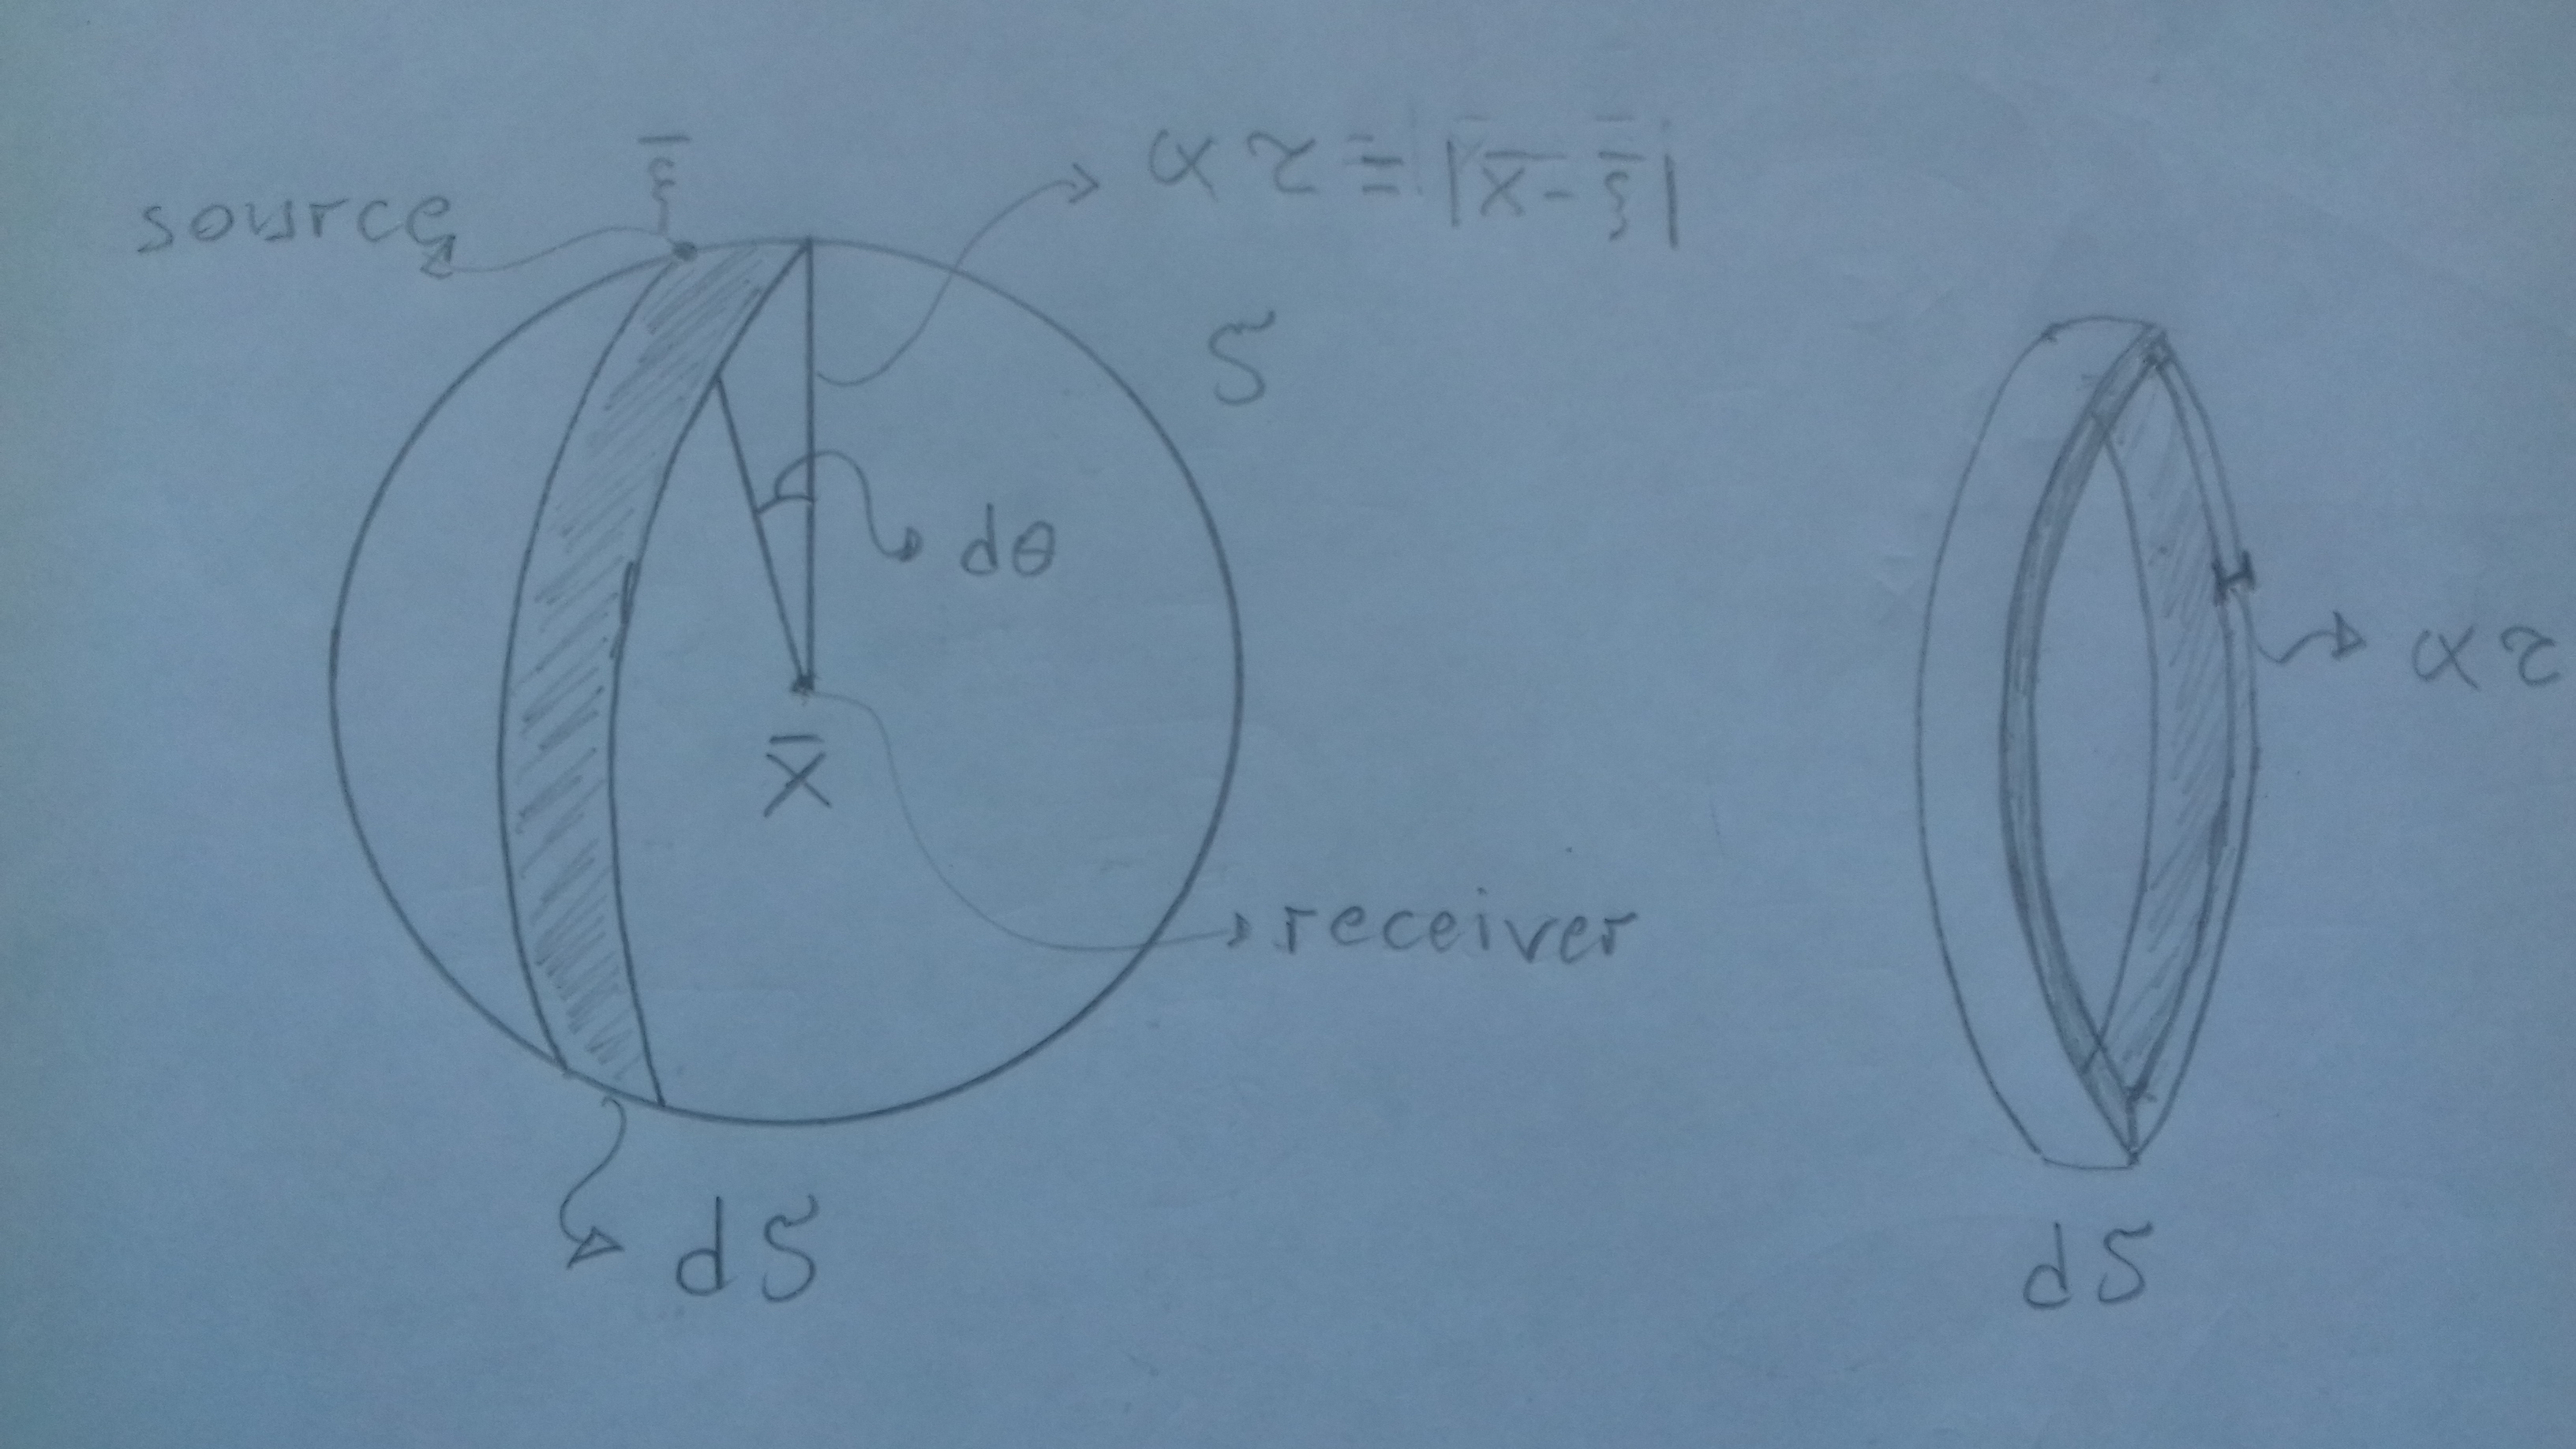
\includegraphics[scale=0.045]{Figura/Fig1.jpg}       
  \end{figure}
  \end{column}
\end{columns}

\begin{flushleft}
Obtemos a seguinte rela\c{c}\~ao:
\end{flushleft}
\begin{eqnarray}
 \int_{V}dV(\eta) &=& \int_{0}^{\infty} \, \alpha \left( \int_{S} dS(\eta) \right) d\tau\, , 
\end{eqnarray}
\begin{flushleft}
onde $\eta$ \'e vari\'avel de integra\c{c}\~ao.
\end{flushleft}


\end{frame}%%%%%%%%%%%%%%%%%%%%%%%%%%%%%%%%%%%%%%%%555



\begin{frame}
\frametitle{\textbf{Solu\c{c}\~ao para a fun\c{c}\~ao de Green em um meio homog\^eneo, isotr\'opico e ilimitado}}

   \begin{flushleft}
     \textcolor{red!60!black}{
     Integrando sobre o volume $V$ atrav\'es de um sistema de cascas esf\'ericas conc\^entricas centradas no ponto de observa\c{c}\~ao:}
   \end{flushleft}        
\begin{eqnarray}
 \int_{V}dV(\eta) &=& \int_{0}^{\infty} \, \alpha \left( \int_{S} dS(\eta) \right) d\tau\, 
\end{eqnarray}

\begin{flushleft}
Por compara\c{c}\~ao re-escrevemos:
\end{flushleft}
\begin{eqnarray}
  \label{ten1}
       \phi(\xvec,t) &=& - \frac{1}{(4\pi\alpha)^{2} \rho}  \int_{-\infty}^{+\infty}\, d\tau \frac{ X_{0} \left( \xivec,t - \tau  \right) }{\tau}  \int_{S}\frac{\partial }{\partial \xi_1} \frac{1}{\left| \xivec \right|} dS\, \\
       \psi(\xvec,t) &=& \frac{1}{(4\pi\beta)^{2} \rho}  \int_{-\infty}^{+\infty}\, d\tau  \frac{ X_{0}  \left( \xivec,t - \tau  \right) }{\tau}    \int_{S} \left(0, \frac{\partial }{\partial \xi_3} \frac{1}{\left| \xivec \right|}, \frac{\partial }{\partial \xi_2} \frac{1}{\left| \xivec \right|} \right) dS \, \nonumber \\
\end{eqnarray}

\end{frame}%%%%%%%%%%%%%%%%%%%%%%%%%%%%%%%%%%%%%%%%555



\begin{frame}
\frametitle{\textbf{Solu\c{c}\~ao para a fun\c{c}\~ao de Green em um meio homog\^eneo, isotr\'opico e ilimitado}}

\begin{flushleft}
    Avaliando a integral de superf\'icie:
\end{flushleft}
\begin{eqnarray}
  \label{ten1}
   h &=& - \int_{S}\frac{\partial }{\partial \eta_{1}} \frac{1}{R} dS(\eta) \, 
\end{eqnarray}

  \begin{columns}        
  \begin{column}{0.15\textwidth}  
  \begin{eqnarray*}
   \alpha\tau &=& \left| \xvec - \xivec \right|\\
   R &=& \left| \xivec -\eta \right|\\
   r &=&  \left| \xvec - \eta \right|
  \end{eqnarray*}
  \end{column}
  \begin{column}{0.75\textwidth}    
  \begin{figure}[h!]   
    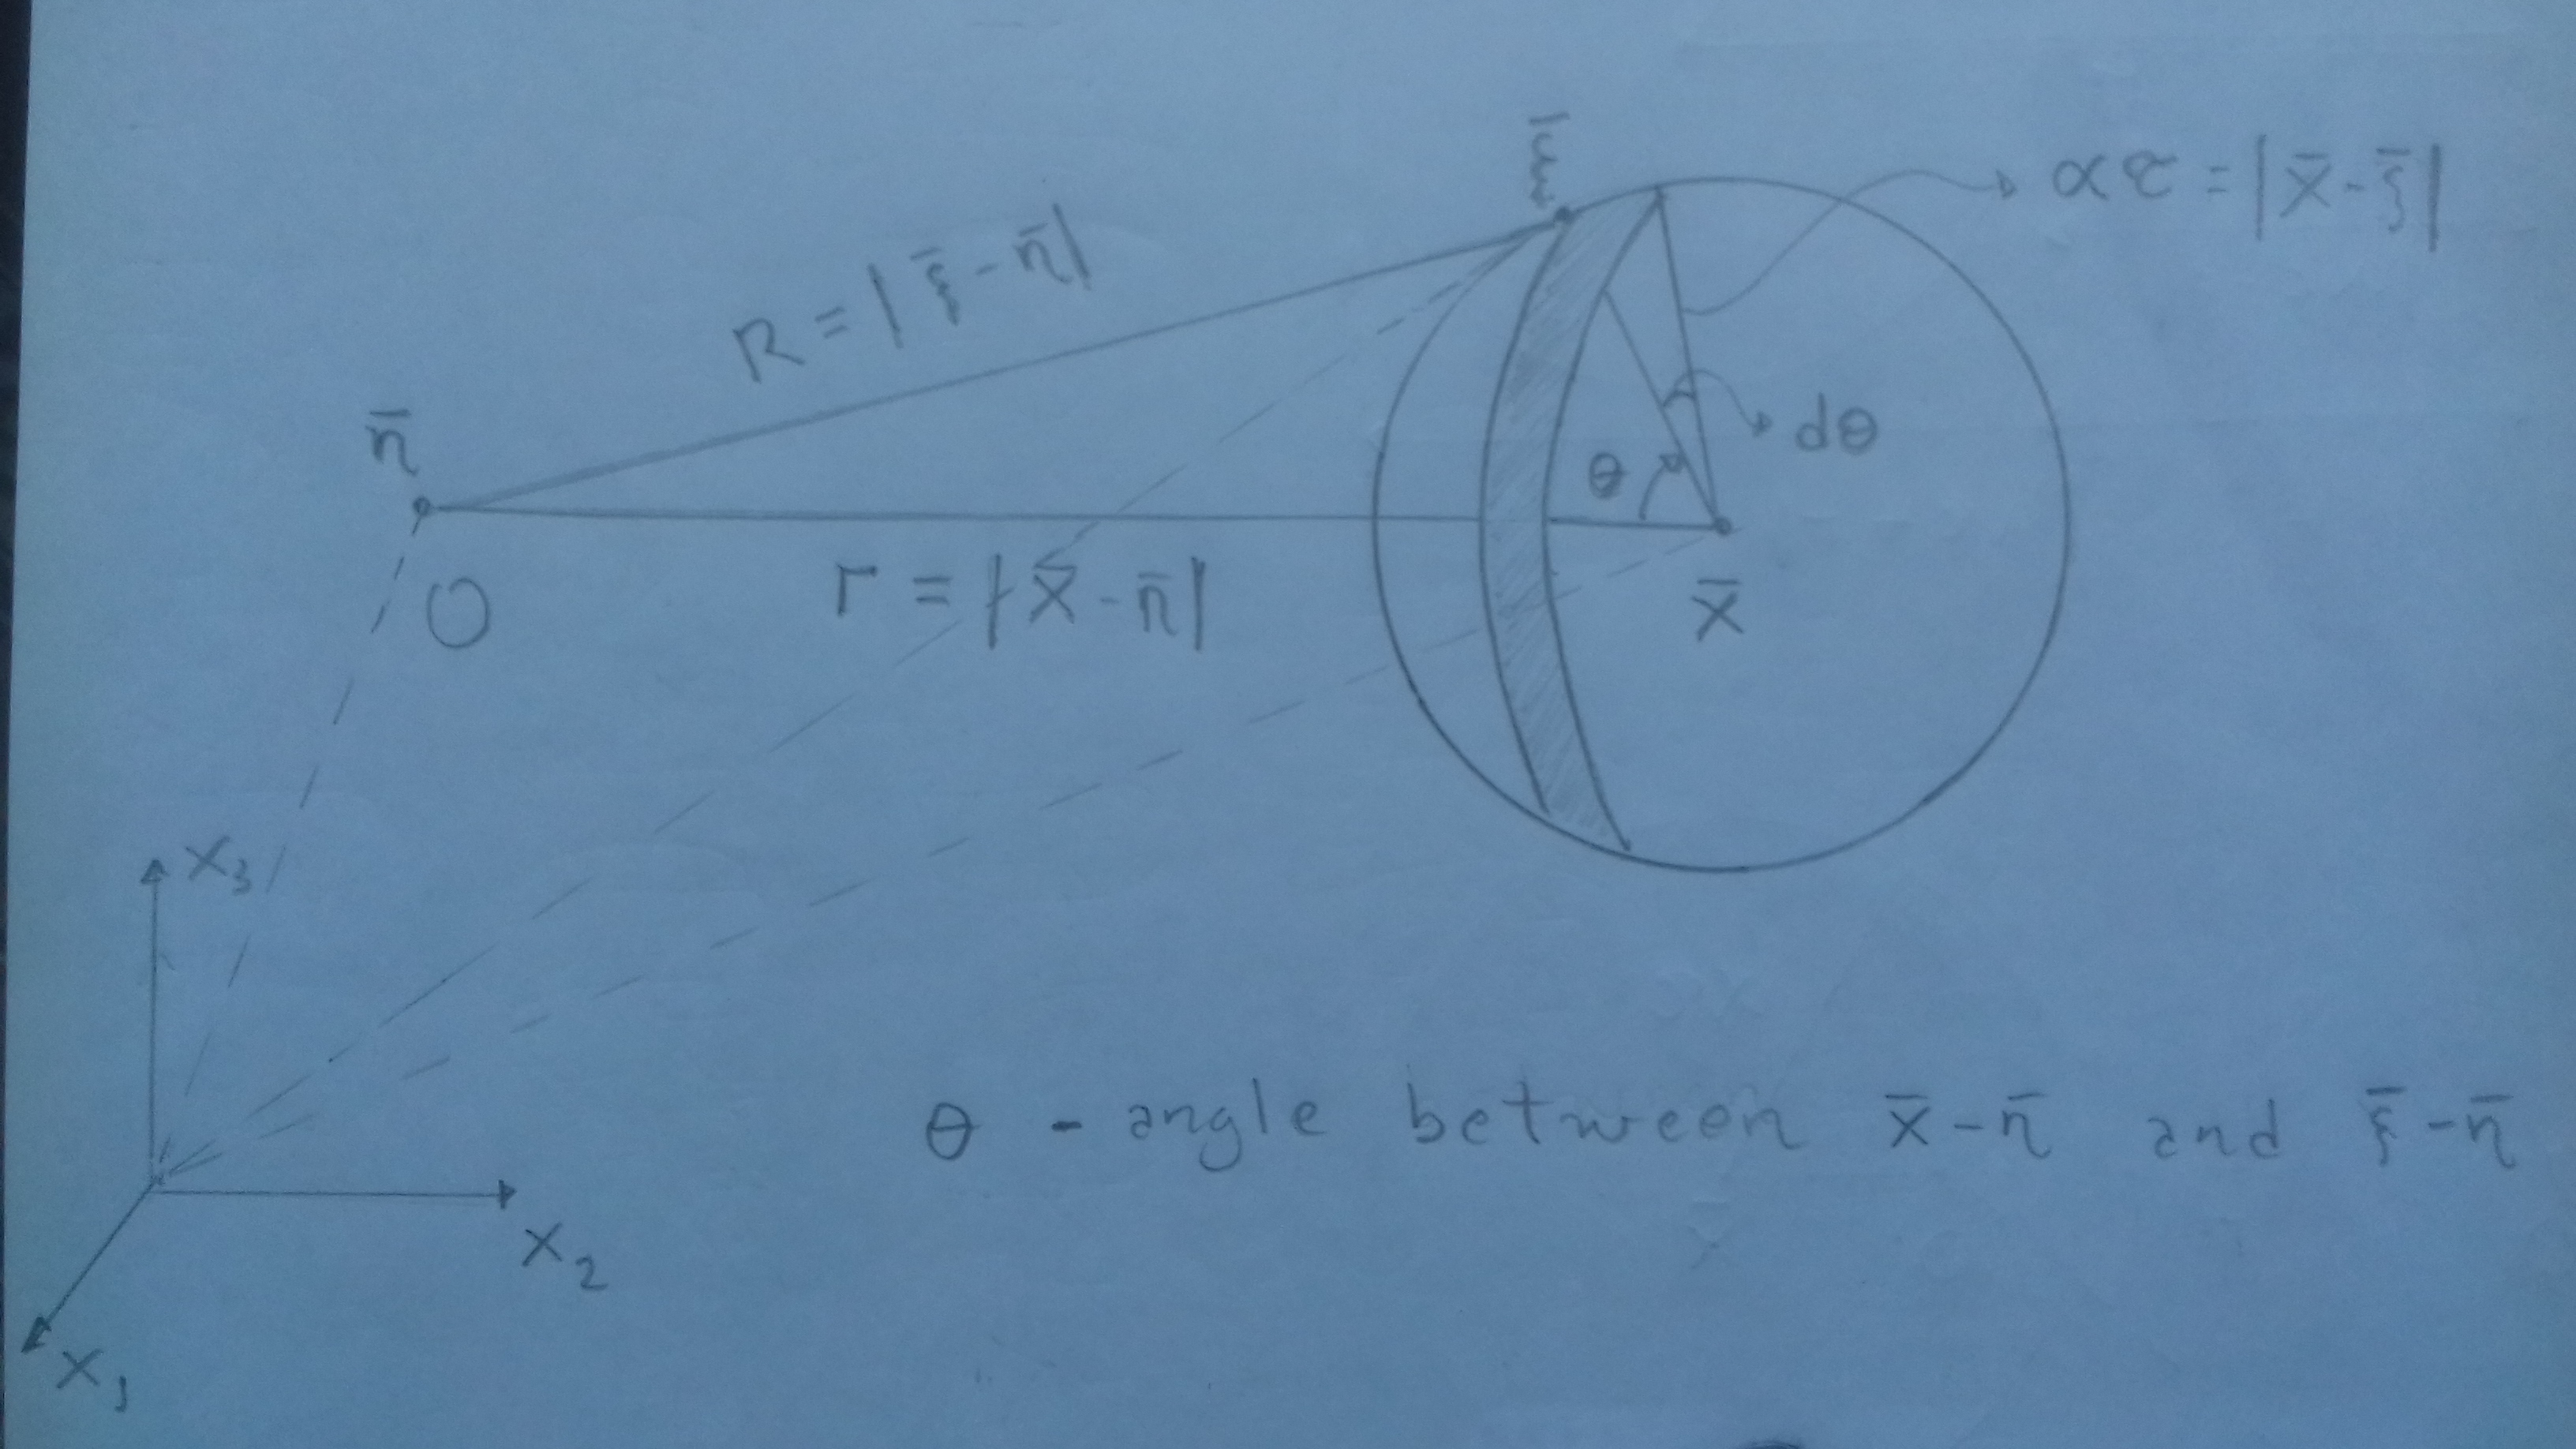
\includegraphics[width=248px, height=120px]{Figura/Fig11.jpg}     
  \end{figure}
  \end{column}
\end{columns}

\end{frame}%%%%%%%%%%%%%%%%%%%%%%%%%%%%%%%%%%%%%%%%555


\begin{frame}
\frametitle{\textbf{Solu\c{c}\~ao para a fun\c{c}\~ao de Green em um meio homog\^eneo, isotr\'opico e ilimitado}}

\begin{flushleft}
     \textcolor{red!60!black}{Avaliando a integral de superf\'icie:}
\end{flushleft}

  \begin{figure}[h!]   
    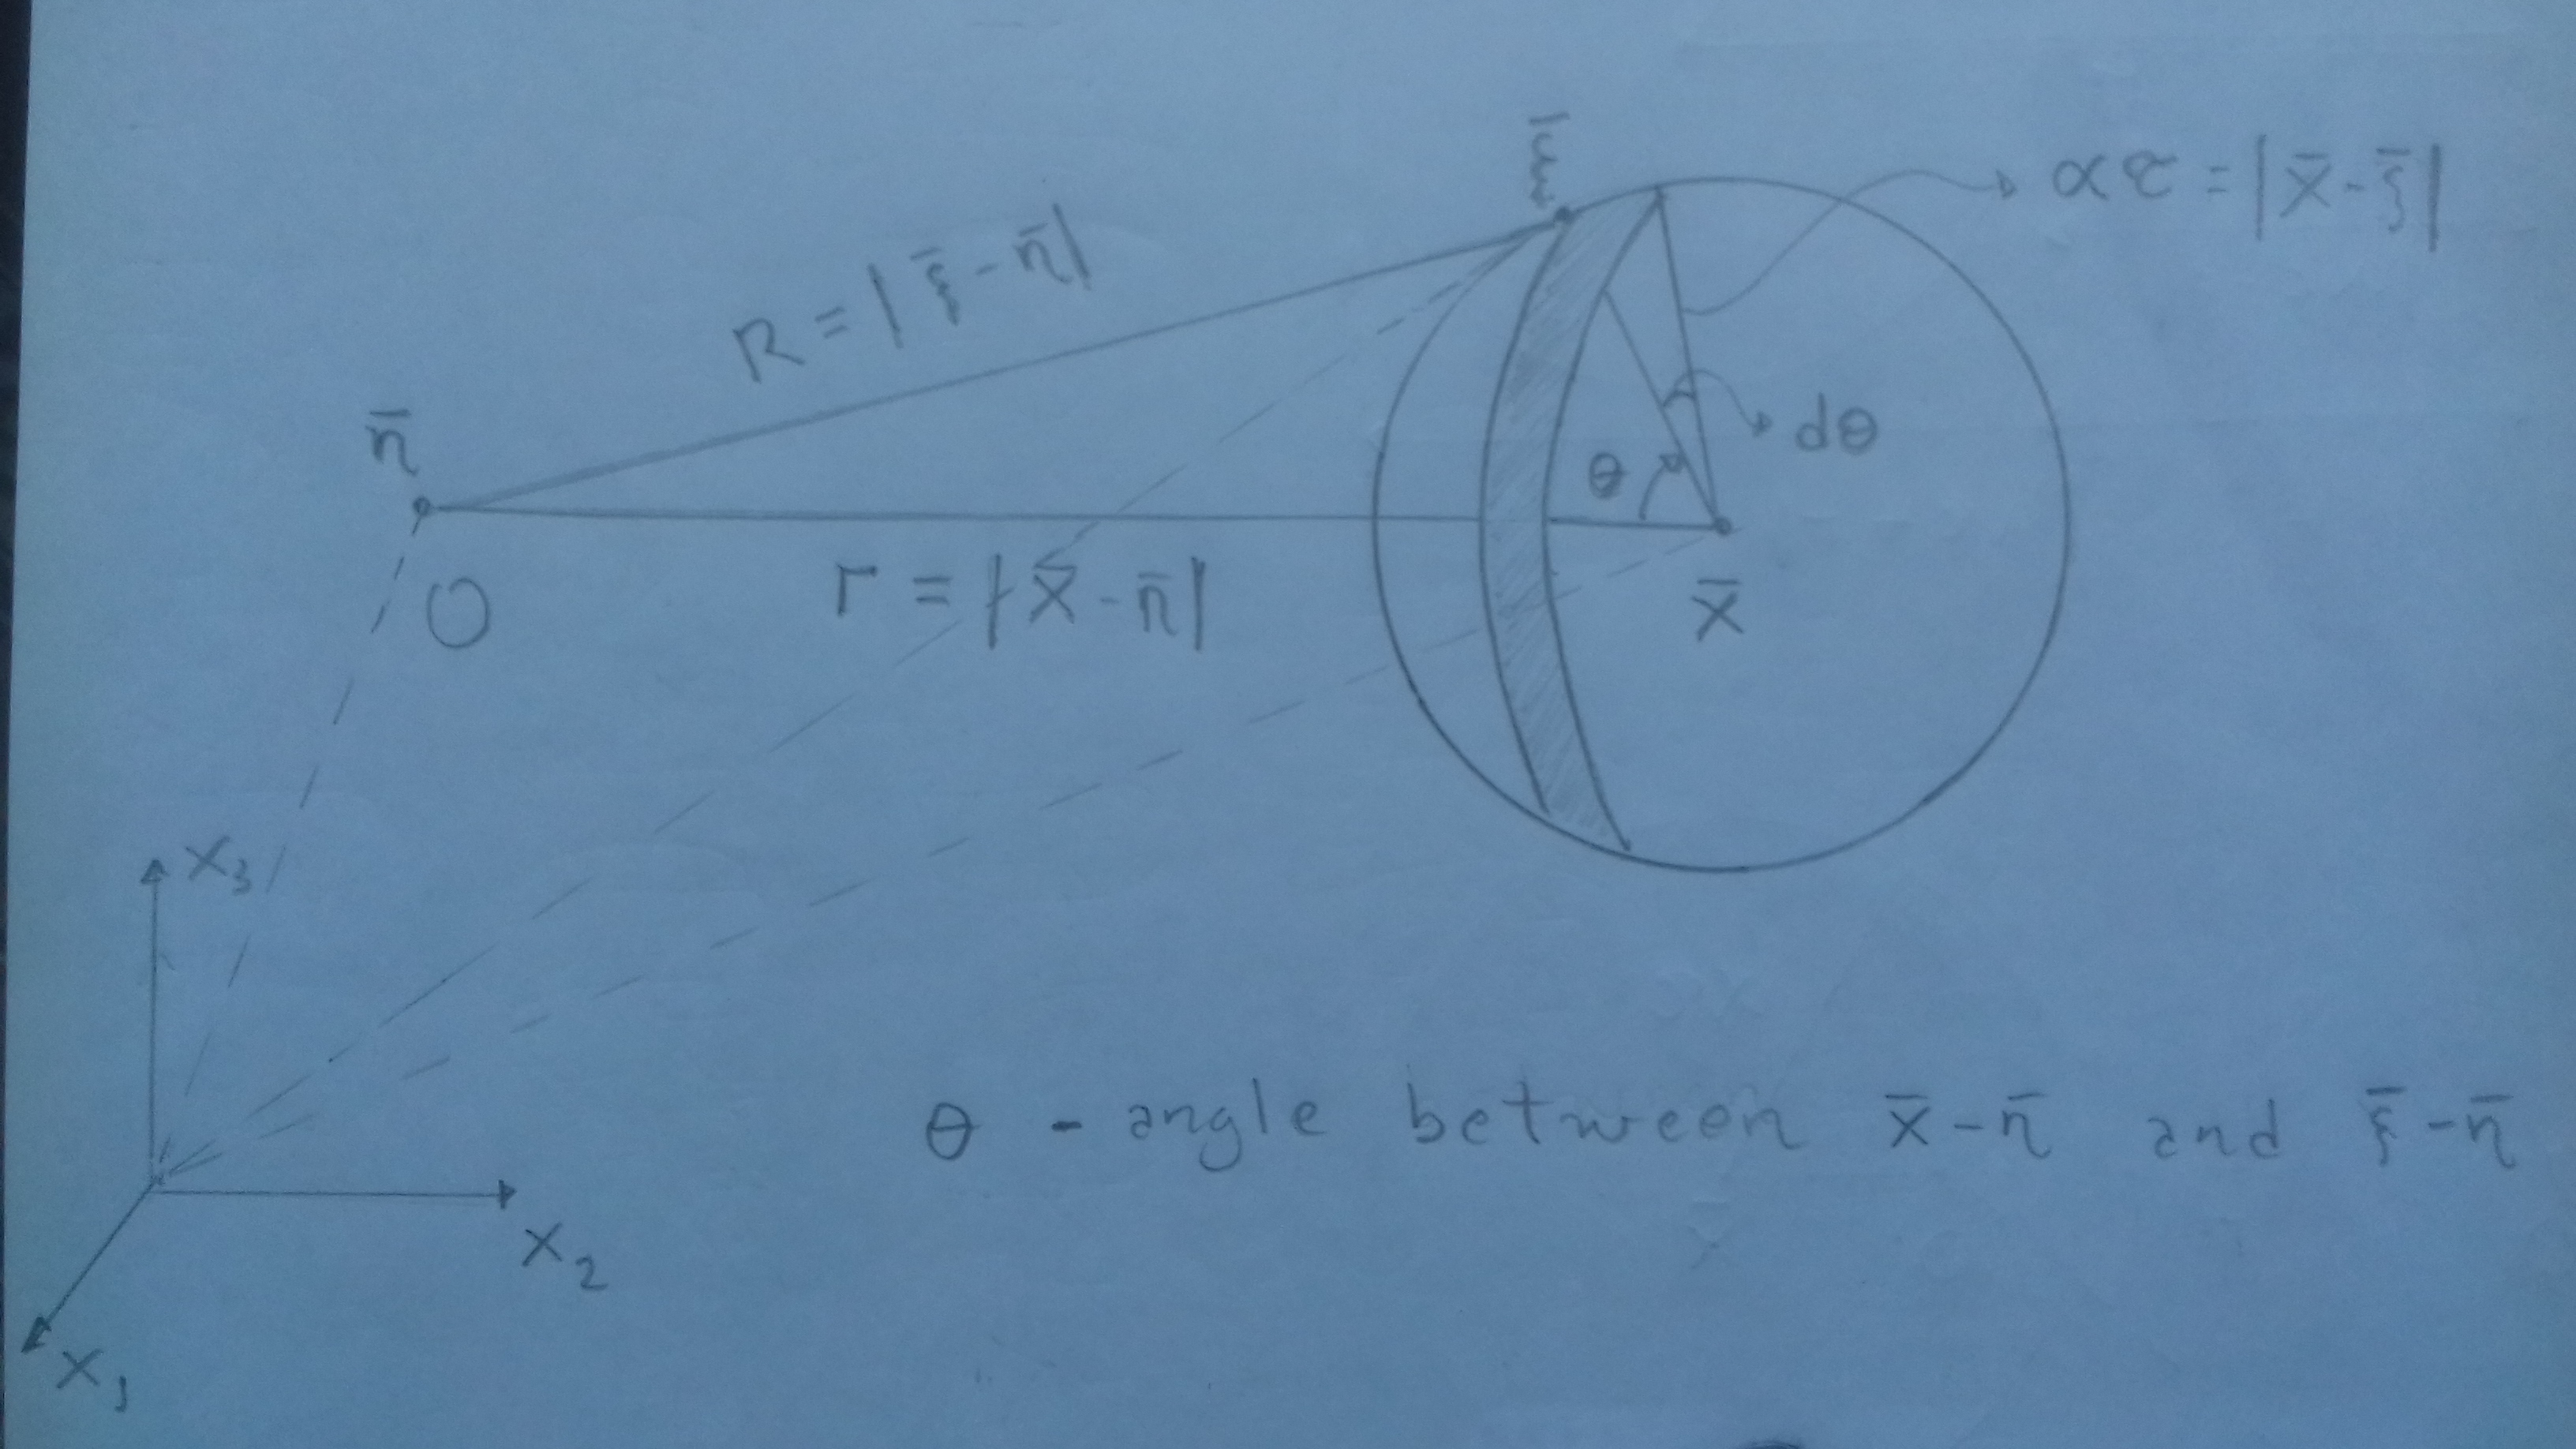
\includegraphics[width=218px, height=100px]{Figura/Fig11.jpg}       
  \end{figure}
\begin{flushleft}
 A vari\'avel integra\c{c}\~ao $\eta$ \'e fixa para todos os pontos $\xivec$ em $S$, 
\end{flushleft}
\begin{eqnarray}
  \label{ten1}
   h &=& - \int_{S}\frac{\partial }{\partial \eta_{1}} \frac{1}{R} dS(\eta)  = - \frac{\partial }{\partial \eta_{1}}\int_{S} \frac{1}{R} dS(\eta) \, 
\end{eqnarray}

\end{frame}%%%%%%%%%%%%%%%%%%%%%%%%%%%%%%%%%%%%%%%%555


\begin{frame}
\frametitle{\textbf{Solu\c{c}\~ao para a fun\c{c}\~ao de Green em um meio homog\^eneo, isotr\'opico e ilimitado}}
\begin{flushleft}
    \textcolor{red!60!black}{Avaliando a integral de superf\'icie:}
\end{flushleft}    

  \begin{figure}[h!]   
  \begin{subfigure}[t]{0.40\linewidth}
    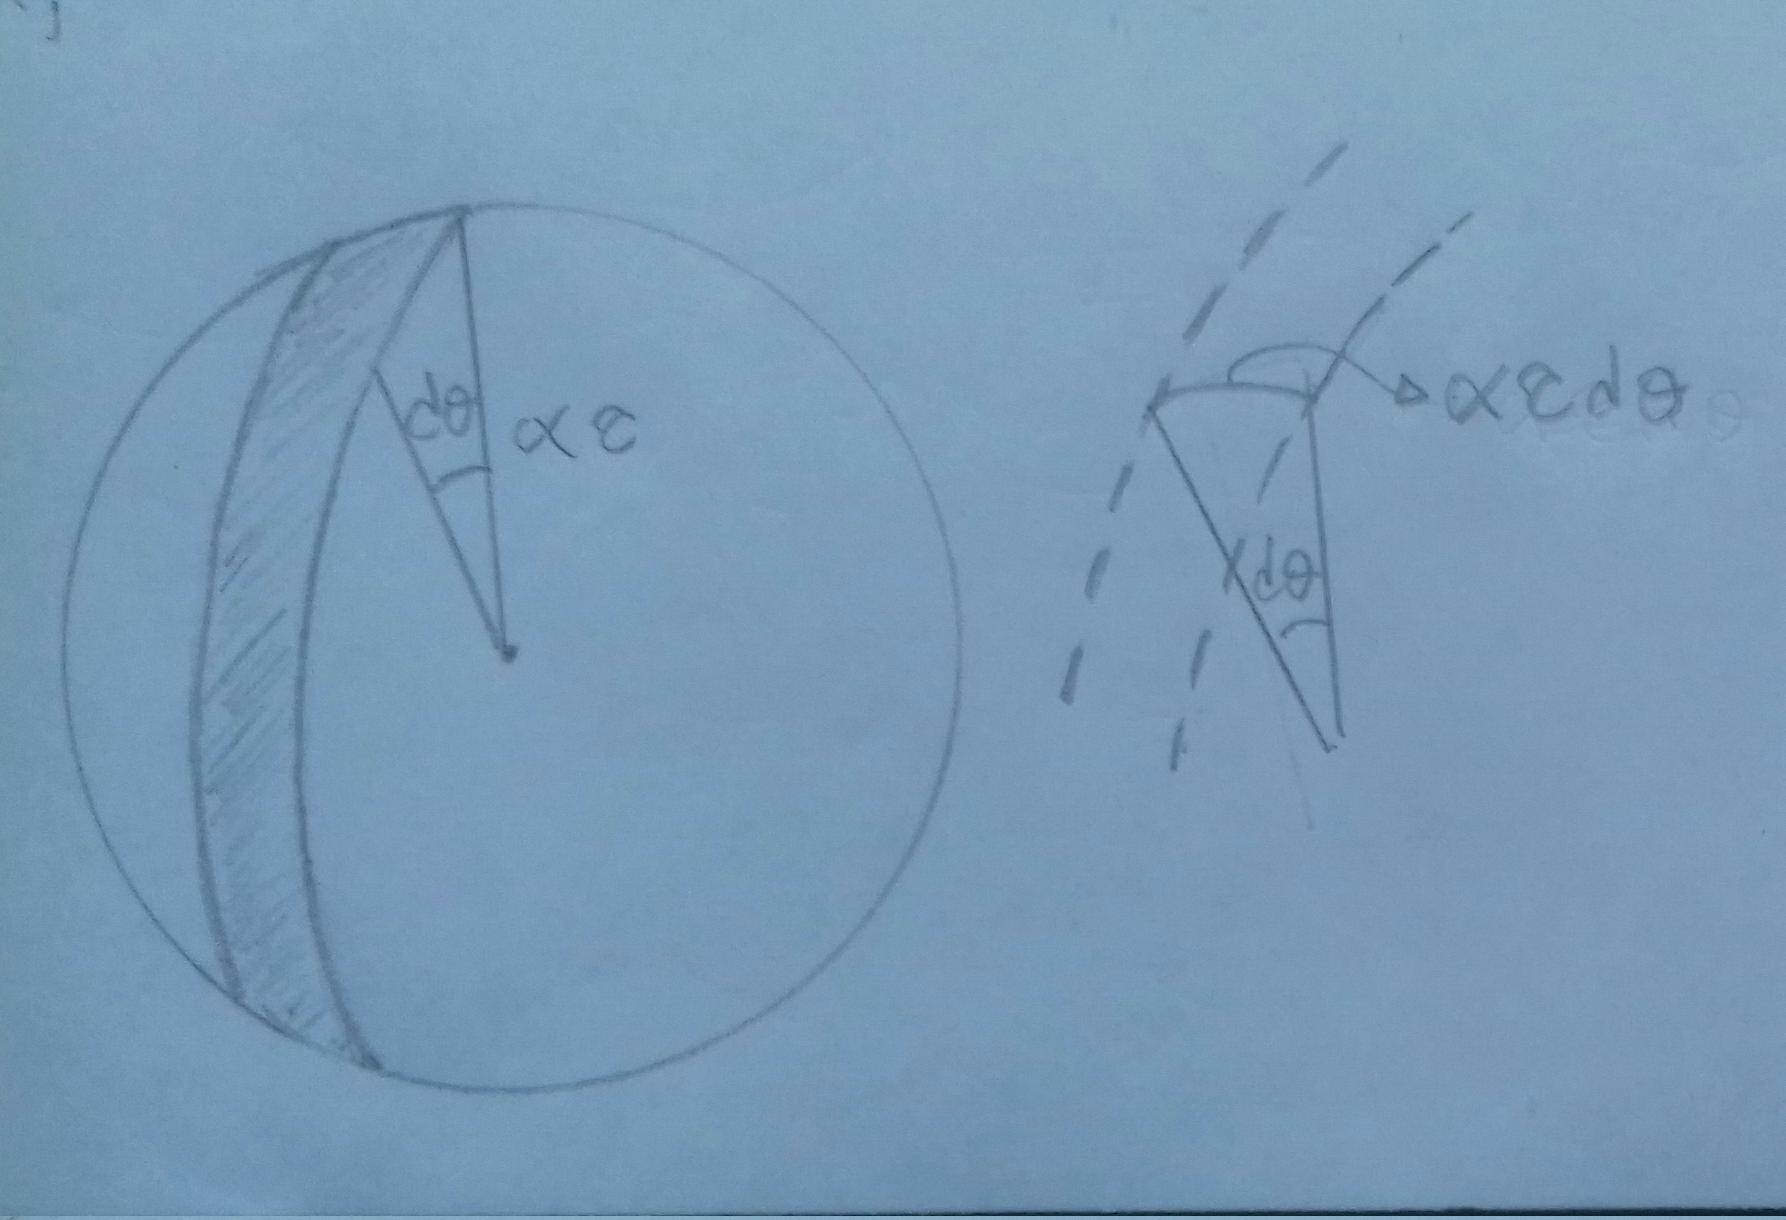
\includegraphics[scale=0.060]{Figura/Fig3.jpg}\\        
  \end{subfigure}  
  \begin{subfigure}[t]{0.40\linewidth}
    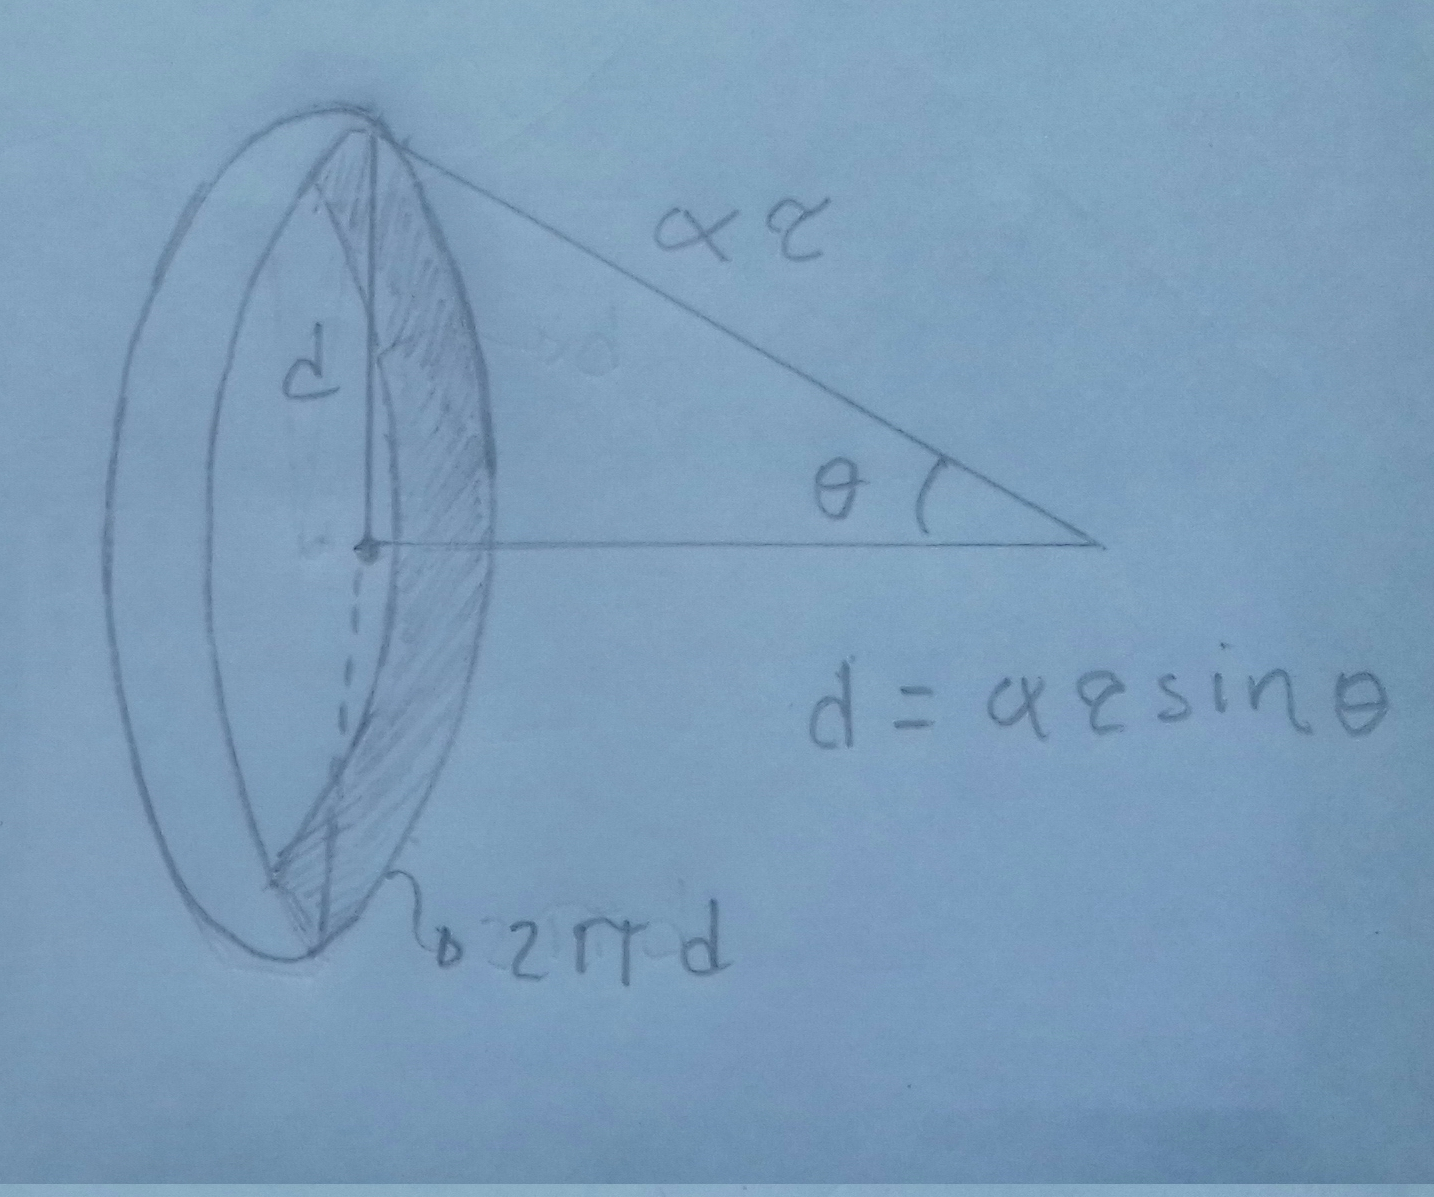
\includegraphics[scale=0.0615]{Figura/Fig4.jpg}\\            
  \end{subfigure}    
  \end{figure}  
\begin{flushleft}
 Um elemento de superf\'icie $dS$ \'e 
\end{flushleft}
\begin{eqnarray}
  \label{ten1}
   dS &=& 2\pi \alpha^2 \tau^2 \sin \theta d\theta \, .
\end{eqnarray}
\begin{flushleft}
 Substituindo o elemento de superf\'icie $dS$,
\end{flushleft}
\begin{eqnarray}
  \label{ten1}
   \int_{S} \frac{1}{R} dS(\eta)  &=& 2\pi \alpha^2 \tau^2 \int_{0}^{\pi} \frac{\sin \theta}{R} d\theta \, 
\end{eqnarray}

\end{frame}%%%%%%%%%%%%%%%%%%%%%%%%%%%%%%%%%%%%%%%%555



\begin{frame}
\frametitle{\textbf{Solu\c{c}\~ao para a fun\c{c}\~ao de Green em um meio homog\^eneo, isotr\'opico e ilimitado}}
\begin{flushleft}
    \textcolor{red!60!black}{Avaliando a integral de superf\'icie:}
\end{flushleft}

\begin{columns}        
  \begin{column}{0.60\textwidth}  
  \begin{figure}[h!]   
    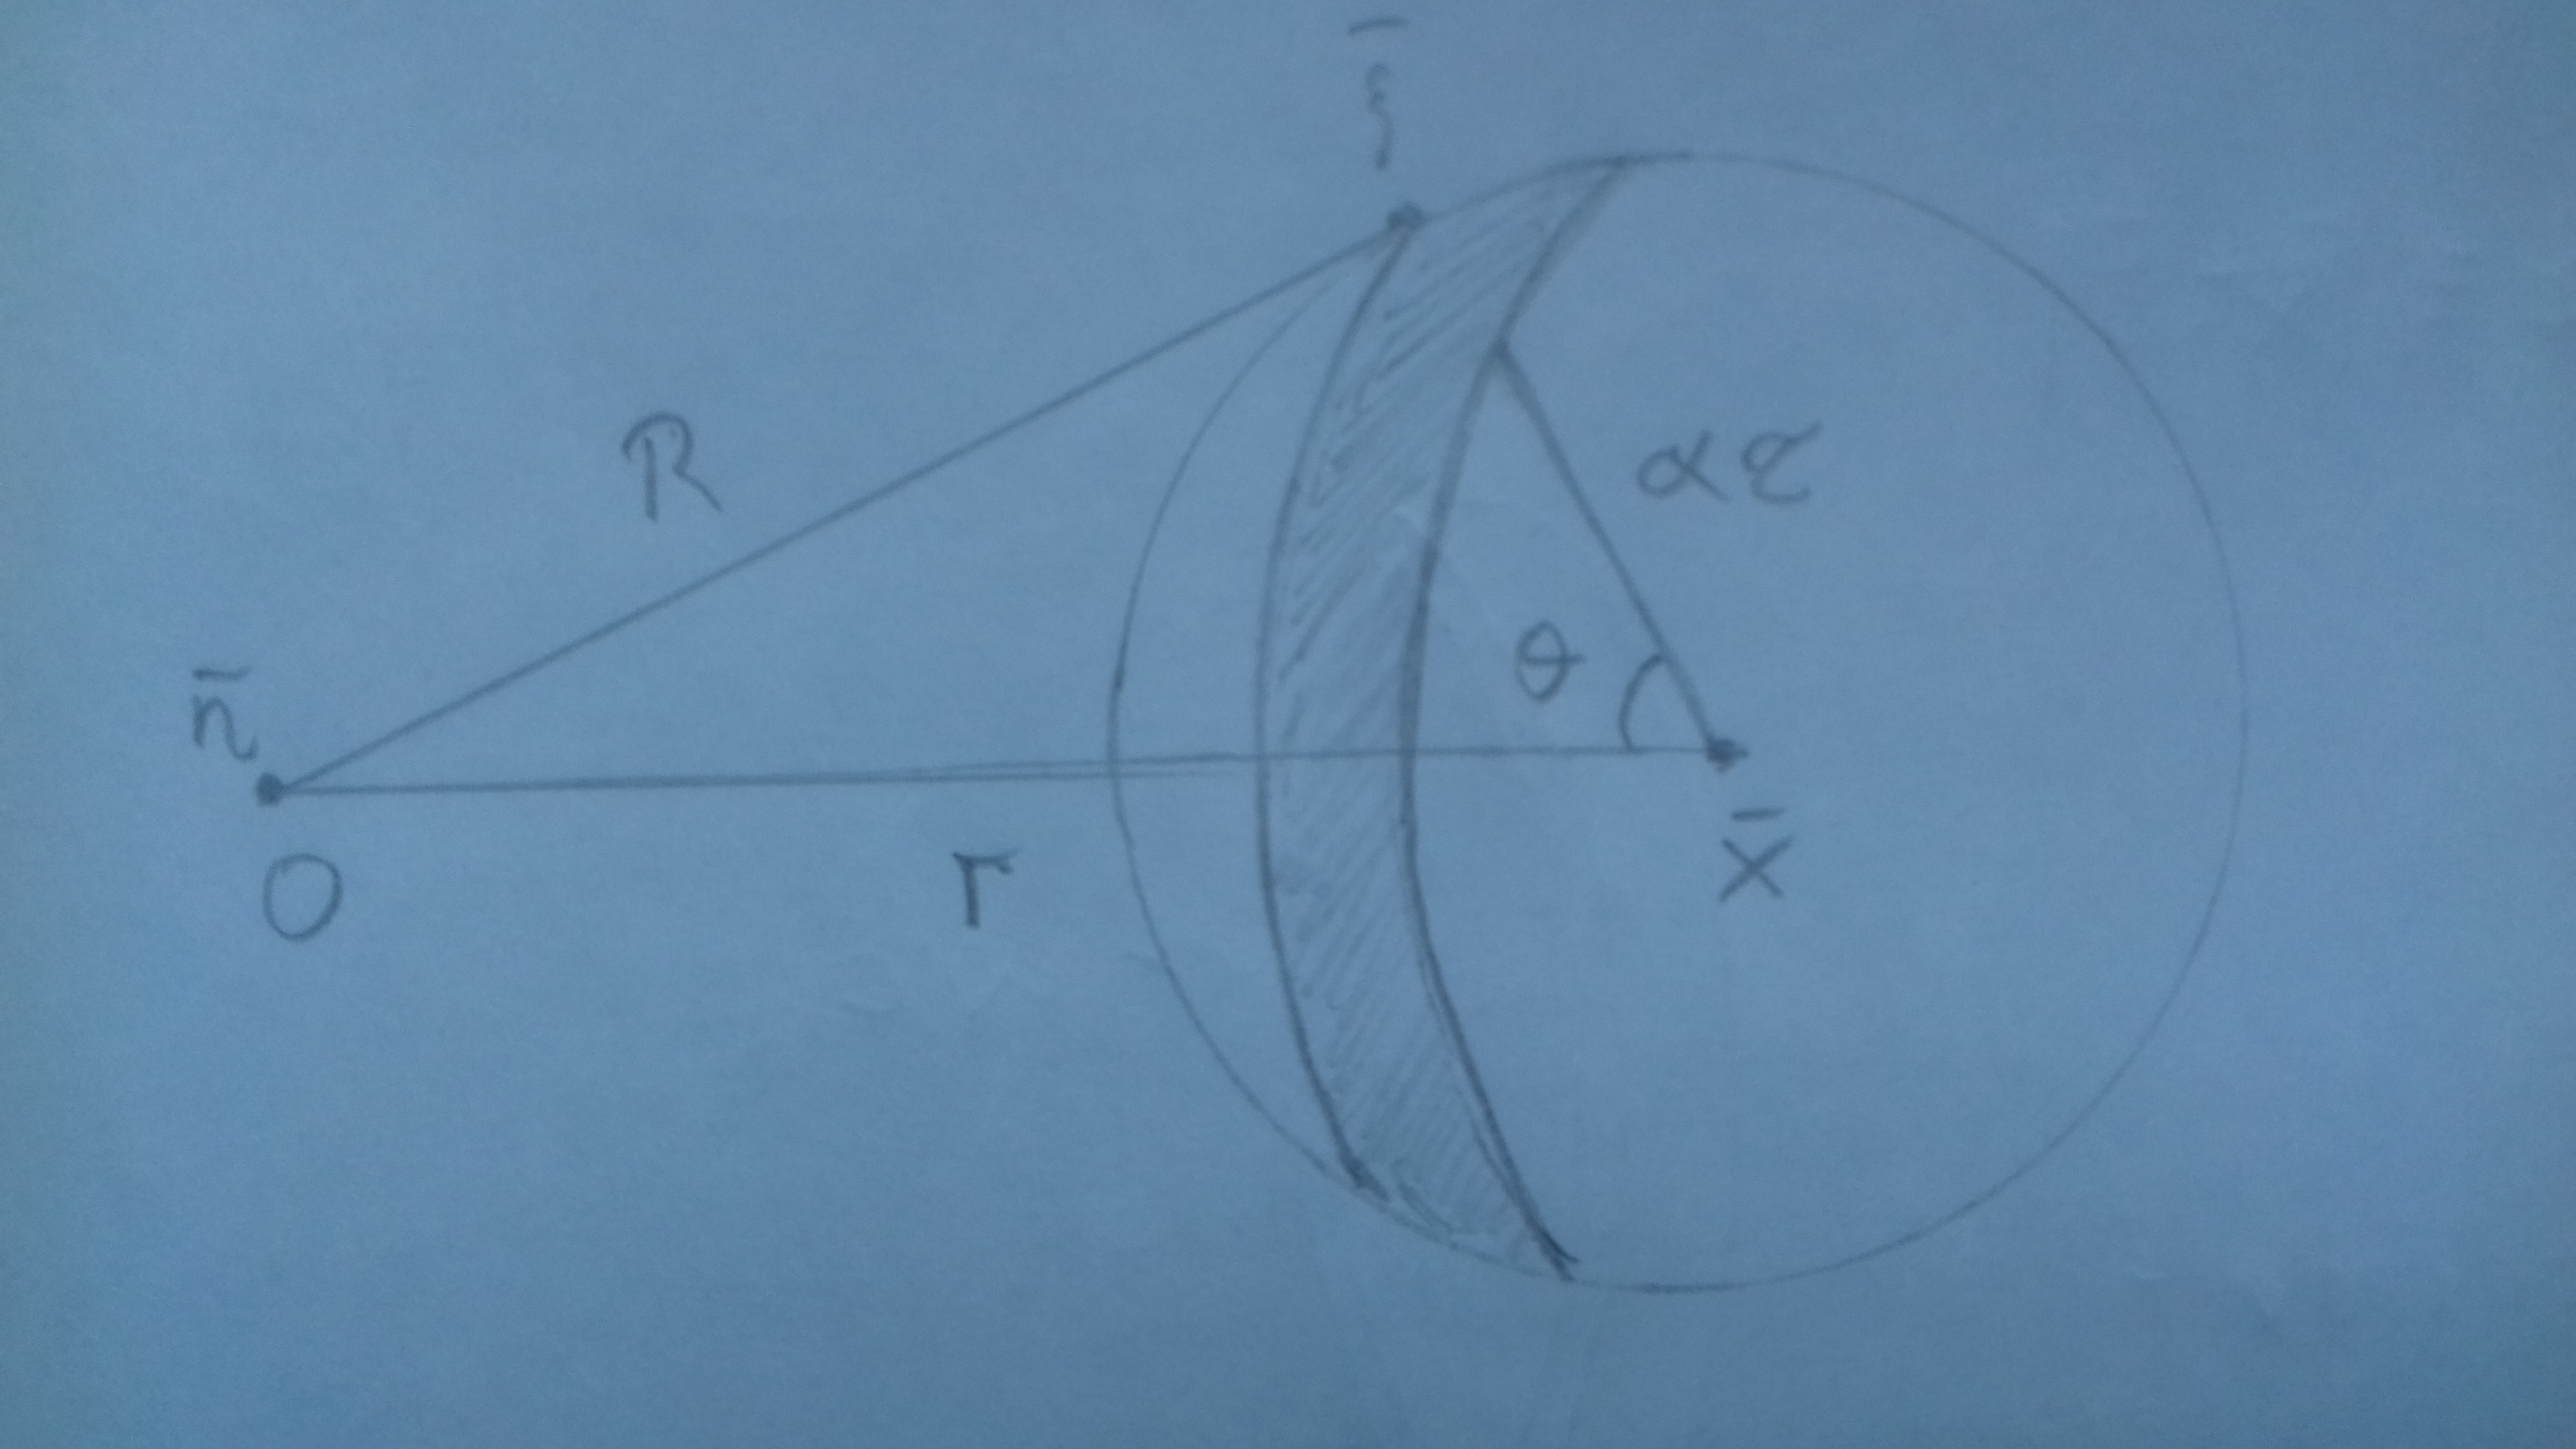
\includegraphics[scale=0.058]{Figura/Fig5.jpg}       
  \end{figure}
  \end{column}
\end{columns}

\begin{flushleft}
 A express\~ao para $\sin \theta d\theta$ usando a lei dos cosenos,
\end{flushleft}
\begin{eqnarray}
  \label{ten1}
   R &=&  r^2 + \alpha^2 \tau^2  - 2r\alpha\tau \cos \theta\,
\end{eqnarray}

\end{frame}%%%%%%%%%%%%%%%%%%%%%%%%%%%%%%%%%%%%%%%%555


\begin{frame}
\frametitle{\textbf{Solu\c{c}\~ao para a fun\c{c}\~ao de Green em um meio homog\^eneo, isotr\'opico e ilimitado}}
\begin{flushleft}
    \textcolor{red!60!black}{Avaliando a integral de superf\'icie:}
\end{flushleft}

\begin{flushleft}
 A express\~ao para $\sin \theta d\theta$ usando a lei dos cosenos,
\end{flushleft}
\begin{eqnarray}
  \label{ten1}
   R &=&  r^2 + \alpha^2 \tau^2  - 2r\alpha\tau \cos \theta\,
\end{eqnarray}
\begin{flushleft}
e tomando o diferencial,
\end{flushleft}
\begin{eqnarray}
  \label{ten1}
   2RdR &=& 2r\alpha\tau \sin \theta d\theta \, .
\end{eqnarray}
\begin{flushleft}
 Substituindo $\sin \theta d\theta$,
\end{flushleft}
\begin{eqnarray}
  \label{ten1}
   \int_{S} \frac{1}{R} dS(\eta)  &=& 2\pi \alpha^2 \tau^2 \int_{0}^{\pi} \frac{\sin \theta}{R} d\theta  = \frac{2\pi \alpha \tau}{r} \int_{\left| \alpha\tau -r \right|}^{\left| \alpha\tau +r \right|}  dR \, 
\end{eqnarray}

\end{frame}%%%%%%%%%%%%%%%%%%%%%%%%%%%%%%%%%%%%%%%%555



\begin{frame}
\frametitle{\textbf{Solu\c{c}\~ao para a fun\c{c}\~ao de Green em um meio homog\^eneo, isotr\'opico e ilimitado}}
\begin{flushleft}
    \textcolor{red!60!black}{Avaliando a integral de superf\'icie:}
\end{flushleft}
\begin{columns}        
  \begin{column}{0.60\textwidth}    
  \begin{figure}[h!]   
    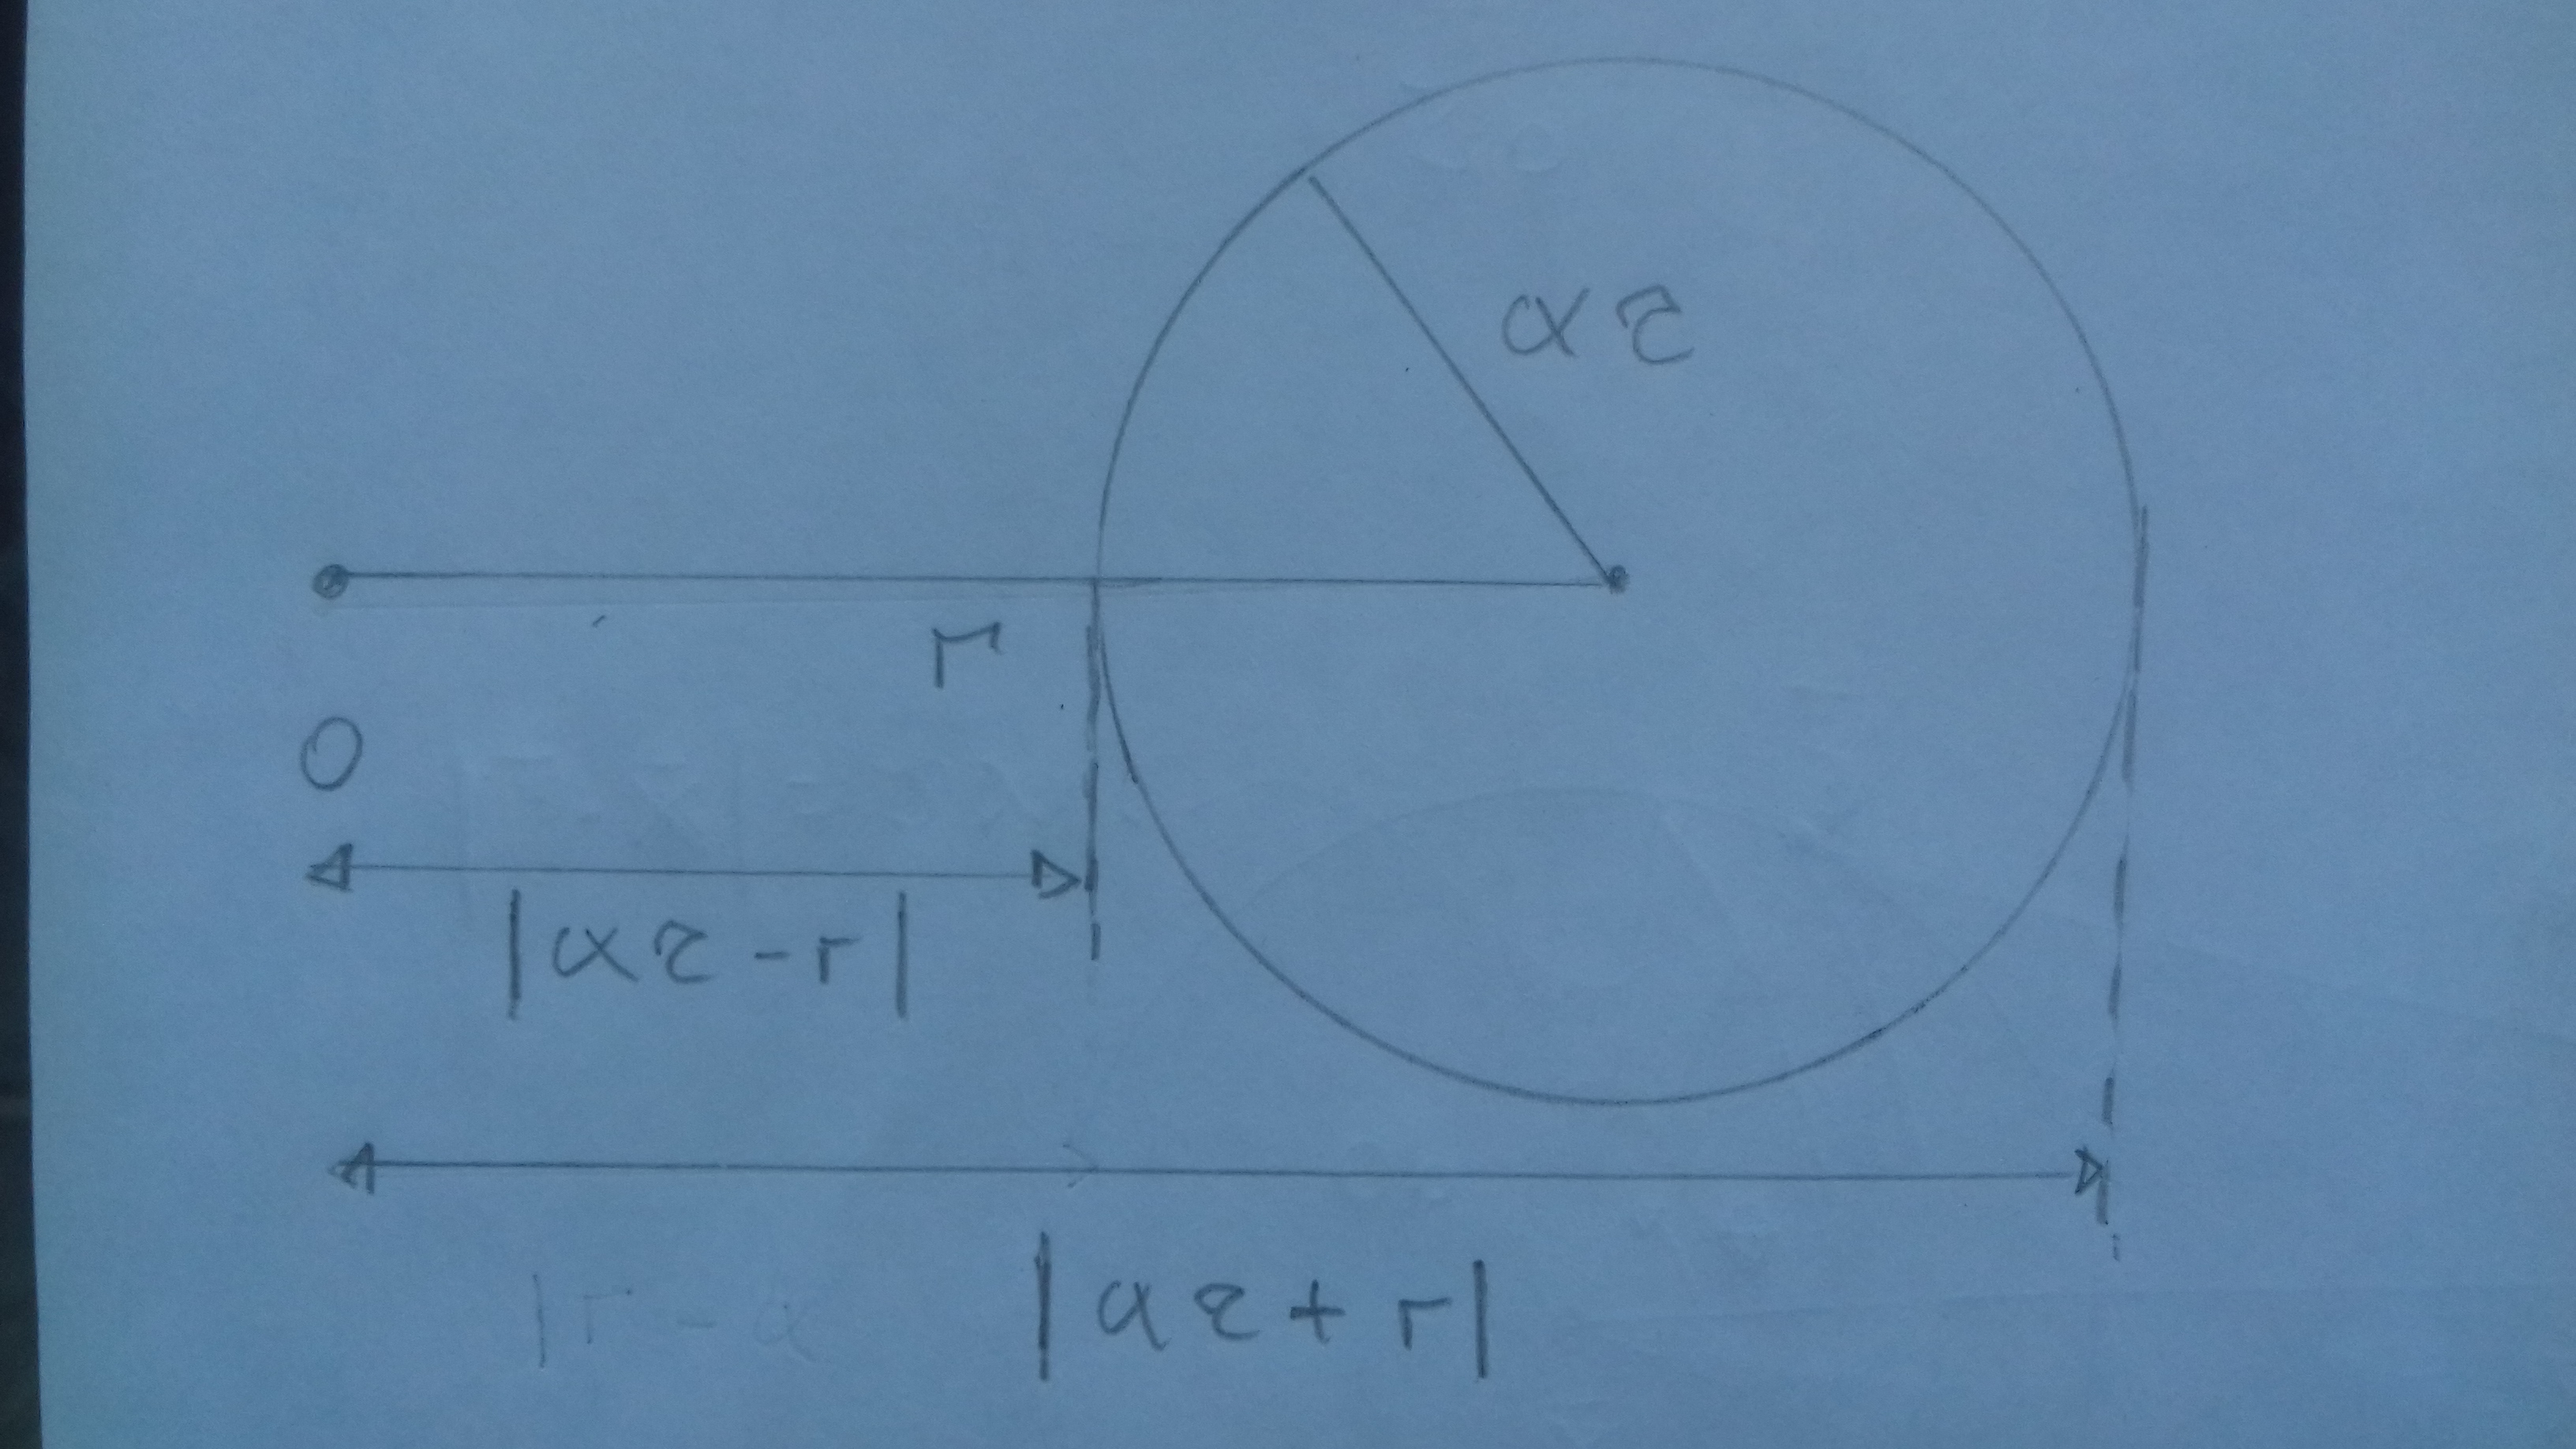
\includegraphics[scale=0.06]{Figura/Fig6}       
  \end{figure}
  \end{column}
\end{columns}

\begin{flushleft}
Agora avaliamos a origem $O$, 
\end{flushleft}
\begin{eqnarray}
  \label{ten1}
   \int_{S} \frac{1}{R} dS(\eta)  &=& \frac{2\pi \alpha \tau}{r} \int_{\left| \alpha\tau -r \right|}^{\left| \alpha\tau +r \right|}  dR  = \frac{2\pi \alpha \tau}{r}\, R \Big|_{\left| \alpha\tau -r \right|}^{\left| \alpha\tau +r \right|} \, 
\end{eqnarray}

\end{frame}%%%%%%%%%%%%%%%%%%%%%%%%%%%%%%%%%%%%%%%%555



\begin{frame}
\frametitle{\textbf{Solu\c{c}\~ao para a fun\c{c}\~ao de Green em um meio homog\^eneo, isotr\'opico e ilimitado}}
\begin{flushleft}
   \textcolor{red!60!black}{Avaliando a integral de superf\'icie:}
\end{flushleft}

\begin{flushleft}
Agora avaliamos a origem $O$, 
\end{flushleft}
\begin{eqnarray}
  \label{ten1}
   \int_{S} \frac{1}{R} dS(\eta)  &=& \frac{2\pi \alpha \tau}{r} \int_{\left| \alpha\tau -r \right|}^{\left| \alpha\tau +r \right|}  dR  = \frac{2\pi \alpha \tau}{r}\, R \Big|_{\left| \alpha\tau -r \right|}^{\left| \alpha\tau +r \right|} \, 
\end{eqnarray}

\begin{itemize}
 \item Se $O$ est\'a dentro de $S$ ($ r/\alpha < \tau $):
 \begin{eqnarray}
  \label{ten1}
   \int_{S} \frac{1}{R} dS &=& \frac{2\pi \alpha \tau}{r}\left[\alpha \tau +r - (\alpha \tau -r )  \right] = 4\pi \alpha \tau
\end{eqnarray}
 \item Se $O$ est\'a fora de $S$ ($  \tau < r/\alpha $):
  \begin{eqnarray}
  \label{ten1}
    \int_{S} \frac{1}{R} dS &=& \frac{2\pi \alpha \tau}{r}\left[\alpha \tau +r - (-\alpha \tau + r )  \right] = \frac{4\pi \alpha^2 \tau^2}{r} 
\end{eqnarray}
\end{itemize}

\end{frame}%%%%%%%%%%%%%%%%%%%%%%%%%%%%%%%%%%%%%%%%555





\begin{frame}
\frametitle{\textbf{Solu\c{c}\~ao para a fun\c{c}\~ao de Green em um meio homog\^eneo, isotr\'opico e ilimitado}}
\begin{flushleft}
   \textcolor{red!60!black}{Avaliando a integral de superf\'icie:}
\end{flushleft}

\begin{itemize}
 \item Se $O$ est\'a dentro de $S$ ($ r/\alpha < \tau $):
 \begin{eqnarray}
  \label{ten1}
    h &=& \frac{\partial}{\partial \eta_1} \left(  4\pi \alpha \tau \right) = 0\, 
\end{eqnarray}
 \item Se $O$ est\'a fora de $S$ ($  \tau < r/\alpha $):
  \begin{eqnarray}
  \label{ten1}
    h &=& \frac{\partial}{\partial \eta_1} \left(  \frac{4\pi \alpha^2 \tau^2}{r} \right) =  4\pi \alpha^2 \tau^2 \frac{\partial}{\partial x_1} \frac{1}{r}\ .   
\end{eqnarray}
\end{itemize}

\end{frame}%%%%%%%%%%%%%%%%%%%%%%%%%%%%%%%%%%%%%%%%555



\begin{frame}
\frametitle{\textbf{Solu\c{c}\~ao para a fun\c{c}\~ao de Green em um meio homog\^eneo, isotr\'opico e ilimitado}}

\begin{flushleft}
Finalmente a integral de superf\'icie tem solu\c{c}\~ao da forma:
\end{flushleft}
\begin{align*}
 \int_{S} \frac{\partial}{\partial x_1 } \frac{1}{\left| \xvec \right| }dS =\begin{cases}
 0  &\mbox{para}\quad  r/\alpha < \tau\\
 4\pi \alpha^2 \tau^2 \frac{\partial }{\partial x_1} \frac{1}{|\xvec|}  &\mbox{para}\quad \tau < r/\alpha
\end{cases}
\end{align*}

\begin{flushleft}
Assim, re-escrevemos as solu\c{c}\~oes das equa\c{c}\~oes do potencial escalar de onda P e 
do potencial vetorial de onda S, respectivamente: 
\end{flushleft}
\begin{eqnarray}
  \label{ten1}
       \phi(\xvec,t) &=& - \frac{1}{4\pi \rho}  \left( \frac{\partial }{\partial x_1} \frac{1}{\left| \xvec\right|} \right)  \int_{0}^{\frac{\left| \xvec\right|}{\alpha}} \tau X_{0}\left( t -\tau \right)  d\tau\, \\
       \psi(\xvec,t) &=& \frac{1}{4\pi\rho}  \left(0, \frac{\partial }{\partial x_3} \frac{1}{\left| \xvec \right|}, -\frac{\partial }{\partial x_2} \frac{1}{\left| \xvec \right|} \right) \int_{0}^{\frac{\left| \xvec\right|}{\beta}} \tau X_{0}\left( t -\tau \right)  d\tau\, 
\end{eqnarray}

\end{frame}%%%%%%%%%%%%%%%%%%%%%%%%%%%%%%%%%%%%%%%%555


\begin{frame}
\frametitle{\textbf{Solu\c{c}\~ao para a fun\c{c}\~ao de Green em um meio homog\^eneo, isotr\'opico e ilimitado}}

\begin{flushleft}
Encontrados os potenciais de Lam\'e $\phi(\xvec,t)$ e $\psi(\xvec,t)$, podemos obter o deslocamento $\uvec(\xvec,t)$ para uma 
fonte do tipo $X_{0}(t)\delta(\xvec)\evec_1$:
\end{flushleft}
\begin{eqnarray}
  \label{ten1}
       \uvec(\xvec,t) &=& \nabla \phi(\xvec,t) + \nabla \times \psi(\xvec,t)\, \\
        &=& \nabla \left[ - \frac{1}{4\pi \rho}  \left( \frac{\partial }{\partial x_1} \frac{1}{\left| \xvec\right|} \right)  \int_{0}^{\frac{\left| \xvec\right|}{\alpha}} \tau X_{0}\left( t -\tau \right)  d\tau  \right] \, \\
        &=& \nabla \times \left[ \frac{1}{4\pi\rho}  \left(0, \frac{\partial }{\partial x_3} \frac{1}{\left| \xvec \right|}, -\frac{\partial }{\partial x_2} \frac{1}{\left| \xvec \right|} \right) \int_{0}^{\frac{\left| \xvec\right|}{\beta}} \tau X_{0}\left( t -\tau \right)  d\tau\right] \, .
\end{eqnarray}

\end{frame}%%%%%%%%%%%%%%%%%%%%%%%%%%%%%%%%%%%%%%%%555


\begin{frame}
\frametitle{\textbf{Solu\c{c}\~ao para a fun\c{c}\~ao de Green em um meio homog\^eneo, isotr\'opico e ilimitado}}

\begin{flushleft}
Encontrados os potenciais de Lam\'e $\phi(\xvec,t)$ e $\psi(\xvec,t)$, podemos obter o deslocamento $\uvec(\xvec,t)$ para uma 
fonte do tipo $X_{0}(t)\delta(\xvec)\evec_1$:
\end{flushleft}
\begin{eqnarray}
  \label{ten1}
       u_i(\xvec,t) &=& 
      \frac{1}{4\pi \rho}  \left( \frac{\partial^2 }{\partial x_i \partial x_1} \frac{1}{r } \right)  \int_{ \frac{r }{\alpha}}^{ \frac{r}{\beta}} \tau X_{0} \left( t -\tau \right)  d\tau\, \\      
       &+& \frac{1}{4\pi \alpha^2 \rho} \frac{1}{r}  \left(\frac{\partial r}{ \partial x_i} \frac{\partial r}{ \partial x_1}  \right)  X_{0} \left(t - \frac{r}{\alpha} \right) \\
       &+& \frac{1}{4\pi\beta^2 \rho} \left( \delta_{i1}  -  \frac{\partial r}{ \partial x_i} \frac{\partial r}{ \partial x_1}  \right) X_{0} \left(t - \frac{r}{\beta} \right)  \, ,
\end{eqnarray}
onde $r = \left| \xvec \right|$.

\end{frame}%%%%%%%%%%%%%%%%%%%%%%%%%%%%%%%%%%%%%%%%555


\begin{frame}
\frametitle{\textbf{Solu\c{c}\~ao para a fun\c{c}\~ao de Green em um meio homog\^eneo, isotr\'opico e ilimitado}}

\begin{flushleft}
Co-senos directores $\gamma_i= (\gamma_1,\gamma_2,\gamma_3)$ para o vetor $\xvec = (x_1,x_2,x_3)$, 
\end{flushleft}
\begin{equation}
 \gamma_1 = \frac{\xvec \cdot \evec_1}{r \left| \evec_1 \right|} = \frac{(x_1,x_2,x_3) \cdot (1,0,0)}{r} = \frac{x_1}{r}
\end{equation}
\begin{flushleft}
e observe que
\end{flushleft}
\begin{equation}
  \frac{\partial r}{\partial x_1} = \frac{\partial }{\partial x_1}\left( \sqrt{x_1^2 + x_2^2 + x_3^2} \right)   =  \frac{x_1}{\sqrt{x_1^2 + x_2^2 + x_3^2}} =  \frac{x_1}{r}
\end{equation}
\begin{flushleft}
Assim,
\end{flushleft}
\begin{equation}
  y_i = \frac{x_i}{r} = \frac{\partial r}{\partial x_i}  
\end{equation}
\begin{flushleft}
De forma an\'aloga, a derivada de $r^{-1}$ em rela\c{c}\~ao $x_j$ e depois em $x_i$ \'e
\end{flushleft}
\begin{equation}
 \frac{\partial^2}{\partial x_i \partial x_j} \frac{1}{r}  = \frac{3\gamma_i\gamma_j - \delta_{ij}}{r^3}\, .
\end{equation}

\end{frame}%%%%%%%%%%%%%%%%%%%%%%%%%%%%%%%%%%%%%%%%555


\begin{frame}
\frametitle{\textbf{Solu\c{c}\~ao para a fun\c{c}\~ao de Green em um meio homog\^eneo, isotr\'opico e ilimitado}}

\begin{flushleft}
\textbf{Solu\c{c}\~ao de Stokes (1849)}: tomando $X_{0}(t)$ como uma for\c{c}a pontual atuando na dire\c{c}\~ao $x_j$ na origem e usando os co-senos 
directores,
\end{flushleft}
\begin{eqnarray*}
  \label{ten1}
       u_i(\xvec,t) &=& X_{0}(t) * G_{ij}(\xvec,t;\xivec,0)\, \\
       &=&\frac{1}{4\pi\rho} \left(3\gamma_i\gamma_j -\delta_{ij} \right) \frac{1}{r^3}  \int_{ \frac{r }{\alpha}}^{ \frac{r}{\beta}} \tau X_{0}\left( t -\tau \right)  d\tau\, \\      
       &+&\frac{1}{4\pi\alpha^2\rho} \gamma_i\gamma_j \,\frac{1}{r}  X_{0}\left(t - \frac{r}{\alpha} \right)\, \\
       &-&\frac{1}{4\pi\beta^2\rho} \left(\gamma_i\gamma_j -\delta_{ij} \right)  \frac{1}{r}  X_{0}\left(t - \frac{r}{\beta} \right)\, .
\end{eqnarray*}
\begin{flushleft}
\end{flushleft}
\end{frame}%%%%%%%%%%%%%%%%%%%%%%%%%%%%%%%%%%%%%%%%555



\begin{frame}
\frametitle{\textbf{Solu\c{c}\~ao para a fun\c{c}\~ao de Green em um meio homog\^eneo, isotr\'opico e ilimitado}}

\begin{flushleft}
\textbf{Solu\c{c}\~ao de Stokes (1849)}: tomando $X_{0}(t)$ como uma for\c{c}a pontual atuando na dire\c{c}\~ao $x_j$ na origem e usando os co-senos 
directores,
\end{flushleft}
\begin{eqnarray*}
  \label{ten1}
       u_i(\xvec,t) &=& X_{0}(t) * G_{ij}(\xvec,t;\xivec,0)\, \\
       &=&\frac{1}{4\pi\rho} \textcolor{red}{\left(3\gamma_i\gamma_j -\delta_{ij} \right) \frac{1}{r^3}  \int_{ \frac{r }{\alpha}}^{ \frac{r}{\beta}} \tau X_{0}\left( t -\tau \right)  d\tau }\, \\      
       &+&\frac{1}{4\pi\alpha^2\rho} \gamma_i\gamma_j \,\frac{1}{r}  X_{0}\left(t - \frac{r}{\alpha} \right)\, \\
       &-&\frac{1}{4\pi\beta^2\rho} \left(\gamma_i\gamma_j -\delta_{ij} \right)  \frac{1}{r}  X_{0}\left(t - \frac{r}{\beta} \right)\, .
\end{eqnarray*}
\begin{flushleft}
\textcolor{red}{Near-field de modo P e S}
\end{flushleft}
\end{frame}%%%%%%%%%%%%%%%%%%%%%%%%%%%%%%%%%%%%%%%%555


\begin{frame}
\frametitle{\textbf{Solu\c{c}\~ao para a fun\c{c}\~ao de Green em um meio homog\^eneo, isotr\'opico e ilimitado}}

\begin{flushleft}
\textbf{Solu\c{c}\~ao de Stokes (1849)}: tomando $X_{0}(t)$ como uma for\c{c}a pontual atuando na dire\c{c}\~ao $x_j$ na origem e usando os co-senos 
directores,
\end{flushleft}
\begin{eqnarray*}
  \label{ten1}
       u_i(\xvec,t) &=& X_{0}(t) * G_{ij}(\xvec,t;\xivec,0)\, \\
       &=&\frac{1}{4\pi\rho} \textcolor{red}{\left(3\gamma_i\gamma_j -\delta_{ij} \right) \frac{1}{r^3}  \int_{ \frac{r }{\alpha}}^{ \frac{r}{\beta}} \tau X_{0}\left( t -\tau \right)  d\tau }\, \\      
       &+&\frac{1}{4\pi\alpha^2\rho} \textcolor{blue}{\gamma_i\gamma_j\, \frac{1}{r}  X_{0}\left(t - \frac{r}{\alpha} \right) }\, \\
       &-&\frac{1}{4\pi\beta^2\rho} \left(\gamma_i\gamma_j -\delta_{ij} \right)  \frac{1}{r}  X_{0}\left(t - \frac{r}{\beta} \right)\, .
\end{eqnarray*}
\begin{flushleft}
\textcolor{red}{Near-field de modo P e S}\hspace{0.5cm}
\textcolor{blue}{Far-field de onda P}
\end{flushleft}
\end{frame}%%%%%%%%%%%%%%%%%%%%%%%%%%%%%%%%%%%%%%%%555


\begin{frame}
\frametitle{\textbf{Solu\c{c}\~ao para a fun\c{c}\~ao de Green em um meio homog\^eneo, isotr\'opico e ilimitado}}

\begin{flushleft}
\textbf{Solu\c{c}\~ao de Stokes (1849)}: tomando $X_{0}(t)$ como uma for\c{c}a pontual atuando na dire\c{c}\~ao $x_j$ na origem e usando os co-senos 
directores,
\end{flushleft}
\begin{eqnarray*}
  \label{ten1}
       u_i(\xvec,t) &=& X_{0}(t) * G_{ij}(\xvec,t;\xivec,0)\, \\
       &=&\frac{1}{4\pi\rho} \textcolor{red}{\left(3\gamma_i\gamma_j -\delta_{ij} \right) \frac{1}{r^3}  \int_{ \frac{r }{\alpha}}^{ \frac{r}{\beta}} \tau X_{0}\left( t -\tau \right)  d\tau }\, \\      
       &+&\frac{1}{4\pi\alpha^2\rho} \textcolor{blue}{\gamma_i\gamma_j\, \frac{1}{r}  X_{0}\left(t - \frac{r}{\alpha} \right) }\, \\
       &-&\frac{1}{4\pi\beta^2\rho} \textcolor{green}{\left(\gamma_i\gamma_j -\delta_{ij} \right)  \frac{1}{r}  X_{0}\left(t - \frac{r}{\beta} \right) }\, .
\end{eqnarray*}
\begin{flushleft}
\textcolor{red}{Near-field de modo P e S} \hspace{0.5cm}
\textcolor{blue}{Far-field de onda P}\hspace{0.5cm}
\textcolor{green}{Far-field de onda S}
\end{flushleft}
\end{frame}%%%%%%%%%%%%%%%%%%%%%%%%%%%%%%%%%%%%%%%%555



\end{document}
